\documentclass{article}

\title{Programmazione di Sistema: OS Internals}
\date{2022-09-28}
\author{Manuel Cadeddu}
\usepackage[italian]{babel}
\usepackage{amsmath}
\usepackage{graphicx}
\usepackage{subcaption}
\usepackage{setspace}
\usepackage{xcolor} 


\begin{document}
	\pagenumbering{arabic}
	\setcounter{tocdepth}{4}
	\setcounter{secnumdepth}{4}
	\maketitle
	\newpage
	\doublespacing
	\tableofcontents
	\singlespacing
	\newpage
	
	\section{Main Memory}

		\subsection{Introduzione}

			\subsubsection{Hardware di Base}
				La Memoria consiste in un array di byte identificati da un indirizzo.
				\\La CPU può accedere solamente alla \textbf{Memoria Centrale} (RAM) e ai \textbf{Registri}, ma non al \textbf{Disco}. Quindi, tutte le istruzioni in esecuzione e i dati che utilizzano devono essere caricati in Memoria prima che la CPU possa operare su essi.
				\\I Registri hanno una memoria molto piccola e veloce ed è possibile accedervi con un solo colpo di clock. Invece, per accedere alla Memoria sono necessari più colpi di ck e questo può causare \textit{stalli}. Per migliorare la situazione sono state introdotte le \textbf{Cache}: buffer di memoria veloce che si trovano nel processore e permettono di non accedere in memoria (se possiedono i dati cercati).
				\\Un problema da gestire è quello di permettere ad un processo di accedere solo alla memoria per la quale è autorizzato. Per farlo si usano solitamente implementazioni hw, perché il SO non interviene negli accessi della CPU alla memoria per motivi di prestazioni.
				\\Una tecnica per implementare questa protezione è quella di avere due registri nella CPU: il \textbf{Base Register} e il \textbf{Limit Register}. Il Base Register contiene l'indirizzo minimo accedibile dal processo, il Limit Register la porzione di memoria assegnata al processo. Quando la CPU deve accedere alla memoria verifica che l'indirizzo sia compreso tra Base e Base + Limit. Se un processo cerca di accedere a un indirizzo non valido, viene generata una \textit{trap} che restituisce il controllo al SO per gestirla.
				\begin{figure}[ht!]
					\centering{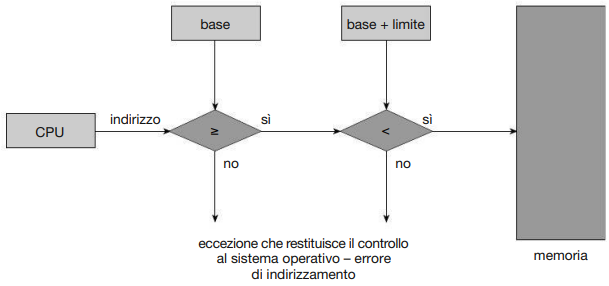
\includegraphics[width=12cm,height=5cm,keepaspectratio]{ch9_1.png}}
				\end{figure}
				\\I Base e Limit Register sono modificabili solo tramite \textit{istruzioni privilegiate} che possono essere eseguite solo in modalità kernel e, poiché solo il SO può essere eseguito in tale modalità, i processi utente non possono modificare il loro valore.

			\newpage
			\subsubsection{Fasi di Elaborazione di un Programma}
				Vediamo i vari componenti che permettono ad un file sorgente di diventare un eseguibile e di essere caricato in RAM per essere eseguito:
				\begin{itemize}
					\item \textbf{preprocessore}: spesso considerato parte del compilatore, permette l'inclusione di header files, di espandere macro, di eseguire compilazione condizionale\dots 
					\\In output si ha un altro file C;
					\item \textbf{compilatore}: traduce il C in linguaggio macchina e produce un \textit{file oggetto} per ogni file C;
					\item \textbf{linker}: unisce i file oggetto e le librerie statiche per creare un \textit{file eseguibile} (\textit{loadable image});
					\item \textbf{loader}: copia la \textit{loadable image} in Memoria, connettendola con librerie dinamiche.
				\end{itemize}
				\begin{figure}[ht!]
					\centering{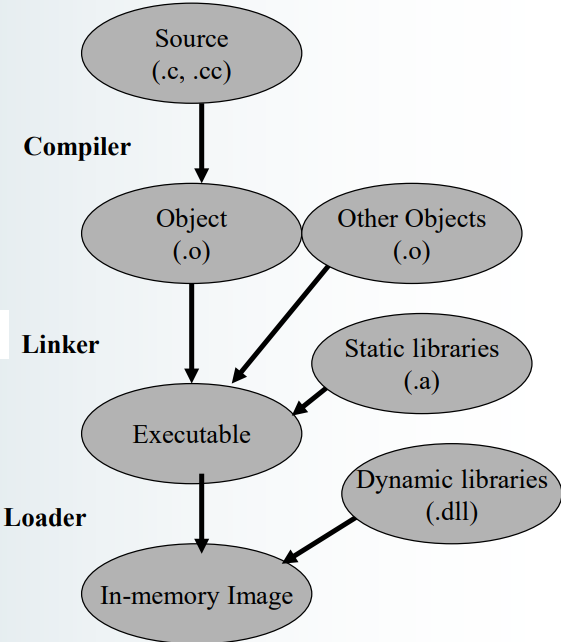
\includegraphics[width=12cm,height=5.5cm,keepaspectratio]{ch9_2.png}}
				\end{figure}
			
			\subsubsection{Address Binding}
				L'Address Binding si rifferisce alla mappatura delle istruzioni e dei dati in posizioni di memoria fisica.
				\\Generalmente, gli indirizzi nel file sorgente sono simbolici (es. nomi variabili), il compilatore associa questi indirizzi simbolici a indirizzi rilocabili (es. 14 byte dall'inizio di questo modulo) e, infine, il linker o il loader genera gli indirizzi assoluti (es. 7014 byte dall'inizio della memoria). Ogni associazione rappresenta una corrispondenza da uno spazio d'indirizzi a un'altro.
				\\Esistono tre tipi di address binding:
				\begin{itemize}
					\item \textbf{Compile Time Address Binding}: se il compilatore sa dove il processo risiederà in memoria, può generare \textbf{codice assoluto}. In questo caso, se dovesse cambiare la locazione iniziale, bisognerebbe ricompilare il codice;
					\item \textbf{Load Time Address Binding}: se in fase di compilazione non è possibile sapere in che punto della memoria risiederà il processo, il compilatore genera \textbf{codice rilocabile}. Nel Load Time Address Binding il \textit{codice assoluto} viene generato in fase di caricamento e, se cambia l'indirizzo del processo, è sufficiente ricaricare il codice per ottenere il nuovo indirizzo "base";
					\item \textbf{Execution Time Address Binding}: se durante l'esecuzione il processo può essere spostato in memoria, si deve ritardare la generazione degli \textit{indirizzi assoluti} fino alla fase di esecuzione. La maggior parte dei SO usa questa soluzione.
				\end{itemize}
		
			\subsubsection{Spazi di Indirizzi Logici e Fisci}
				Un indirizzo generato dalla CPU è normalmente chiamato \textbf{indirizzo logico}, mentre quello caricato nel MAR (Memory Address Register) è chiamato \textbf{indirizzo fisico}. Le tecniche di binding degli indirizzi in fase di compilazione e di caricamento producono indirizzi logici e fisici identici, quella in fase di esecuzione no. In questo caso ci si riferisce agli indirizzi logici col termine \textbf{indirizzi virtuali}.
				\\L'insieme degli indirizzi logici generati da un programma forma lo \textbf{spazio degli indirizzi logici}; l'insieme degli indirizzi fisici corrispondenti a tali indirizzi logici è lo \textbf{spazio degli indirizzi fisci}.
				\\Per implementare l'Execution Time Address Binding,  l'associazione dagli indirizzi virtuali a quelli fisici è svolta da un dispositivo interno alla CPU: l'\textbf{MMU} (\textbf{Memory Management Unit}). Come vedremo più avanti, questo binding può essere realizzato in diversi modi. Per esempio, sommando l'indirizzo logico al contenuto del registro base (ora chimato \textbf{relocation register}).
				\begin{figure}[ht!]
					\centering{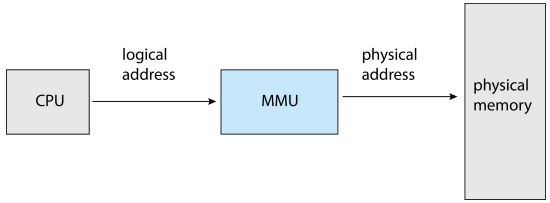
\includegraphics[width=12cm,height=3.5cm,keepaspectratio]{ch9_3.png}}
				\end{figure}

			\subsubsection{Dynamic Loading}
				Nella discussione svolta fin’ora, era necessario che l’intero programma e i dati di un processo fossero in RAM perché il processo potesse essere eseguito. Per migliorare l’utilizzo della memoria si può ricorrere al \textbf{caricamento dinamico} (dynamic loading): prima di tutto si carica il programma principale in memoria e, quando una procedura ne richiama un’altra, innanzitutto si controlla che quella richiesta sia stata caricata. Se non lo è, viene caricata e vengono aggiornate le tabelle degli indirizzi del programma. A questo punto il controllo passa alla procedura appena caricata. Notare che tutte le procedure si tengono su disco in un formato di caricamento rilocabile.
				\\Il caricamento dinamico non richiede un supporto particolare del SO. Spetta agli utenti progettare i programmi in modo da trarre vantaggio da un metodo di questo tipo. Il SO può tuttavia aiutare il programmatore fornendo librerie di procedure che realizzano il caricamento dinamico.
			

			\subsubsection{Dynamic Linking e Librerie Condivise}
				Le \textbf{Dynamically Linked Libraries} (\textbf{DLLs}, librerie caricate dinamicamente) sono librerie di sistema che vengono collegate ai programmi utente quando questi vengono eseguiti. Alcuni SO consentono solo il collegamento statico (static linking), in cui le librerie di sistema sono trattate come qualsiasi altro modulo oggetto e combinate dal caricatore nell’immagine binaria del programma. Il concetto di linking dinamico, invece, è analogo a quello di dynamic loading. Invece di differire il caricamento di una procedura fino al momento dell’esecuzione, si differisce il collegamento. Questa caratteristica si usa soprattutto con le librerie di sistema, per esempio le librerie di subroutine del linguaggio. Senza questo strumento tutti i programmi di un sistema dovrebbero disporre, all’interno dell’eseguibile, di una copia della libreria di linguaggio (o almeno delle procedure cui il programma fa riferimento). Tutto ciò spreca spazio nei dischi e in memoria centrale.
				\\Con il linking dinamico, invece, per ogni riferimento a una procedura di libreria s’inserisce all’interno dell’eseguibile una piccola porzione di codice di riferimento (\textbf{stub}), che indica come localizzare la giusta procedura di libreria residente in memoria o come caricare la libreria se la procedura non è già presente. Durante l’esecuzione, lo stub controlla se la procedura richiesta è già in memoria, altrimenti provvede a caricarla; in entrambi i casi lo stub sostituisce se stesso con l’indirizzo della procedura, che viene poi eseguita. In questo modo, quando si raggiunge nuovamente quel segmento del codice, si esegue direttamente la procedura di libreria, senza costi aggiuntivi per il linking dinamico. Con questo metodo tutti i processi che usano una libreria del linguaggio eseguono la stessa copia del codice della libreria. Questo sistema è noto anche con il nome di \textbf{librerie condivise}.
				\\A differenza del caricamento dinamico, il linking dinamico e le librerie condivise richiedono generalmente l’assistenza del sistema operativo. Se i processi presenti in memoria sono protetti l’uno dall’altro, il sistema operativo è l’unica entità che può controllare se la procedura richiesta da un processo è nello spazio di memoria di un altro processo, o che può consentire l’accesso di più processi agli stessi indirizzi di memoria.

		\subsection{Allocazione Contigua della Memoria}
			La memoria centrale deve contenere sia il SO che i vari processi, quindi bisogna gestirla in modo efficiente. Vediamo ora la prima tecnica per l'allocazione della memoria: l'\textbf{allocazione contigua della memoria}.
			\\La RAM viene di solito divisa in due partizioni, una per il SO e una per i processi. Poiché l'IVT si trova solitamente agli indirizzi inferiori, anche il SO viene allocato agli indirizzi più bassi.
			\\Con l’allocazione contigua della memoria, ciascun processo è contenuto in una singola sezione di memoria contigua a quella che contiene il processo successivo. Per assicurarsi che si acceda alla memoria corretta è possibile utilizzare i registri Base e Limit:
			\begin{figure}[ht!]
				\centering{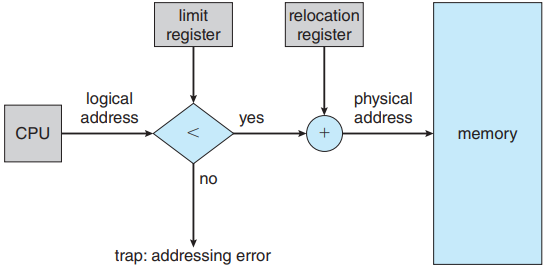
\includegraphics[width=12cm,height=4cm,keepaspectratio]{ch9_4.png}}
			\end{figure}
			\\L'utilizzo di questi registri può risultare util anche per cambiare dinamicamente la dimensione della memoria dedicata al processo (non sempre possibile).

			\subsubsection{Allocazione della Memoria}
				Uno dei metodi più semplici per l’allocazione della memoria consiste nel suddividere la stessa in partizioni di dimensione fissa.
				\\Nello schema a partizione variabile il SO conserva una tabella in cui sono indicate le partizioni di memoria disponibili e quelle occupate. Inizialmente
				tutta la memoria è a disposizione dei processi utenti; si tratta di un grande blocco di memoria disponibile, un buco (\textbf{hole}). Nel lungo periodo la memoria contiene una serie di buchi di diverse dimensioni.
				\begin{figure}[ht!]
					\centering{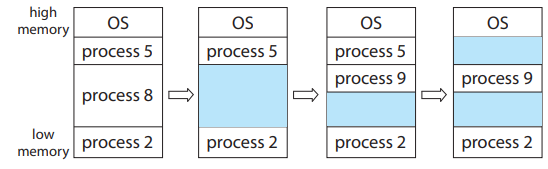
\includegraphics[width=12cm,height=3cm,keepaspectratio]{ch9_5.png}}
				\end{figure}
				\\Quando entrano nel sistema, i processi vengono inseriti in una coda d’ingresso. Per determinare a quali processi si debba assegnare la memoria, il SO tiene conto dei requisiti di memoria di ciascun processo e della quantità di spazio di
				memoria disponibile. Quando a un processo si assegna dello spazio, il processo stesso viene caricato in memoria e può quindi competere per il controllo della CPU. Al termine, rilascia la memoria che gli era stata assegnata, e il SO può impiegarla per un altro processo presente nella coda d’ingresso.
				\\I criteri più usati per scegliere un buco libero tra quelli disponibili nell’insieme sono i seguenti:
				\begin{itemize}
					\item \textbf{Firstfit}: si assegna il primo buco abbastanza grande. La ricerca può cominciare sia dall’inizio dell’insieme di buchi sia dal punto in cui era terminata la ricerca precedente. Si può fermare la ricerca non appena s’individua un buco libero di dimensioni sufficientemente grandi;
					\item \textbf{Bestfit}: si assegna il più piccolo buco in grado di contenere il processo. Si deve
					compiere la ricerca in tutta la lista, a meno che questa non sia ordinata per dimensione. Tale criterio produce le parti di buco inutilizzate più piccole;
					\item \textbf{Worstfit}: si assegna il buco più grande. Anche in questo caso si deve esaminare tutta la lista, a meno che non sia ordinata per dimensione. Tale criterio produce le	parti di buco inutilizzate più grandi, che possono essere più utili delle parti più
					piccole ottenute col criterio best-fit.
				\end{itemize}
				Con l’uso di simulazioni si è dimostrato che sia first-fit sia best-fit sono migliori rispetto a worst-fit in termini di risparmio di tempo e di utilizzo di memoria. D’altra parte nessuno dei due è chiaramente migliore dell’altro per quel che riguarda l’utilizzo della memoria ma, in genere, first-fit è più veloce.

			\subsubsection{Frammentazione}
				Si distinguono:
				\begin{itemize}
					\item \textbf{frammentazione esterna}: spazio libero in RAM tra i diversi processi;
					\item \textbf{frammentazione interna}: memoria non occupata dal processo che però è stata allocata per esso.
				\end{itemize}
				La frammentazione esterna dipende dalla dimensione della memoria e da quella dei processi ma è generalmente abbastanza grave. Con l'algoritmo first-fit, per esempio, l'analisi statistica rivela che per \textit{n} blocchi, si perdono circa 0.5*\textit{n} blocchi (\textbf{regola del 50 per cento}), ovvero 1/3 della memoria non viene usato.
				\\Un metodo per migliorare il problema della frammentazione esterna è quello della \textbf{compattazione}: si spostano i blocchi di memoria dedicati ai processi creando un unico grande blocco. Questo però non deve essere possibile solo in fase di assemblaggio o loading, ma anche mentre i processi sono in esecuzione (in READY). Quindi gli indirizzi devono essere rilocabili dinamicamente. Se lo sono, la rilocazione richiede solo lo spostamento del programma e dei dati, e quindi la modifica del registro di rilocazione in modo che possieda il nuovo Base Register. La compattazione può però generare il \textit{problema I/O}, ovvero se un processo viene spostato mentre è in WAIT, in attesa di un operazione di I/O, la scrittura/lettura può essere fatta nella porzione di memoria sbagliata. Per risolvere questo problema sono possibili due soluzioni: impedire lo spostamento di processi che stanno eseguendo operazioni I/O o utilizzare dei buffer del SO, non soggetti a reallocazione, come intermediari tra la memoria e i dispositivi I/O.
				\\L'algoritmo di compattazione più semplice consiste nello spostare tutti i processi verso un'estremità della memoria e può essere assai oneroso. 
				\\Altre due tecniche usate per evitare la frammentazione esterna sono la \textbf{segmentazione} e la \textbf{paginazione} (queste tecniche si possono combinare).

		\subsection{Paginazione}
			La paginazione è una tecnica che permette l'assegnazione di blocchi di memomoria non contigui ad un processo. La paginazione evita la frammentazione esterna e la necessità di compattare perché non c'è più il problema di avere blocchi di memoria di dimensioni variabili. 
			\\Il metodo di base consiste nello suddividere la \underline{memoria fisica} in blocchi di dimensione fissa, chiamati \textbf{frame}, e la \underline{memoria logica} in blocchi della stessa dimensione (dei frame), detti \textbf{pagine}. Quando si deve eseguire un processo, si caricano le sue pagine nei frame disponibili, prendendole dalla memoria ausiliaria o dal file system. Questa tecnica fornisce grandi funzionalità. Per esempio, ora lo spazio degli indirizzi logici è totalmente separato dallo spazio degli indirizzi fisici e dunque un processo può avere uno spazio degli indirizzi logici a 64 bit anche se il sistema ha meno di $2^{64}$ byte di memoria fisica.
			\\Gli indirizzi logici vengono divisi in \textbf{page number} (\textbf{p}) e \textbf{page offset} (\textbf{d} = displacement). Il \textit{page number} serve come indice per la \textbf{paging table}, contenente l'indice del frame, che viene usato per calcolare l'indirizzo fisico.
			\\L'hardware di supporto è il seguente:
			\begin{figure}[ht!]
				\centering{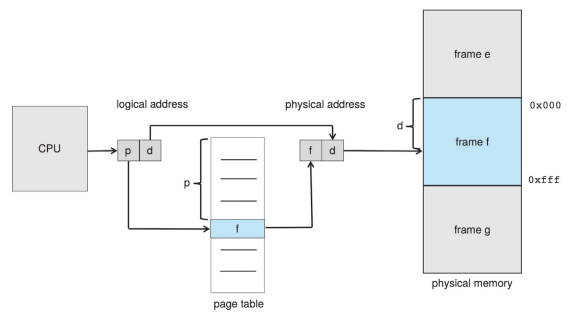
\includegraphics[width=12cm,height=6.5cm,keepaspectratio]{ch9_6.png}}
			\end{figure}
			\\La dimensione di una pagina, così come quella di un frame, è definita dall’hardware ed è, in genere, una potenza di 2 compresa tra 512 byte e 1 Gb. La scelta di una potenza di 2 facilita la traduzione di un indirizzo logico nei corrispondenti numero e offset di pagina. Se la dimensione dello spazio degli indirizzi logici (dimensione memoria logica) è \textit{$2^{m}$} byte (servono indirizzi di \textit{m} bit per identificare un determinato byte) e la dimensione di una pagina è di \textit{$2^{n}$} byte (servono indirizzi di n bit per identificare un determinato byte), per identificare una pagina servono indirizzi di \textit{m} - \textit{n} bit ($2^{m}$/$2^{n}$ pagine).
			\\L’indirizzo logico ha quindi la seguente forma:
			\begin{figure}[ht!]
				\centering{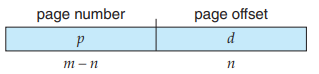
\includegraphics[width=12cm,height=1.3cm,keepaspectratio]{ch9_8.png}}
			\end{figure}
			\\dove \textit{p} è un indice della tabella delle pagine e
			\textit{d} è l’offset all’interno della pagina.
			\\Vediamo un esempio. Consideriamo la seguente memoria:
			\begin{figure}[ht!]
				\centering{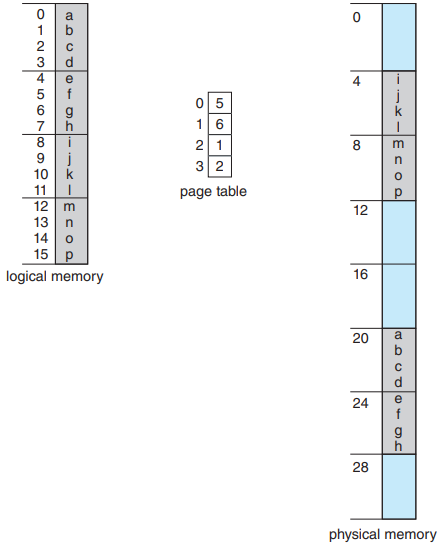
\includegraphics[width=12cm,height=6cm,keepaspectratio]{ch9_9.png}}
			\end{figure}
			\\Possiamo osservare che: \textit{m} = 4, \textit{n} = 2 e che la memoria fisica può contenere 8 frame. Per ottenere l'indirizzo fisico si calcola \textit{f} moltiplicando il numero di pagina indicato nella tabella delle pagine per la dimensione della pagina e si somma \textit{d} al risutato.

			\subsubsection{Frammentazione Interna}
				Con la paginazione si evita la frammentazione esterna ma non quella interna. Infatti, poiché la dimensione dei processi solitamente non è un multiplo di quella dei frame, l'ultimo frame può essere riempito solo parzialmente:
				\begin{itemize}
					\item caso migliore: 0 byte;
					\item caso peggiore: dim\_frame - 1 byte;
					\item caso medio: dim\_frame/2;
				\end{itemize}
				Da queste considerazioni possiamo osservare che più le pagine sono piccole, minore è la frammentazione interna ma maggiore è la dimensione della page table. Attualmente la dimensione tipica delle pagine è compresa tra 4 e 8 KB.

			\subsubsection{Struttura Entry della Page Table}
				La entry di una Page Table mantiene le seguenti informazioni:
				\begin{figure}[ht!]
					\centering{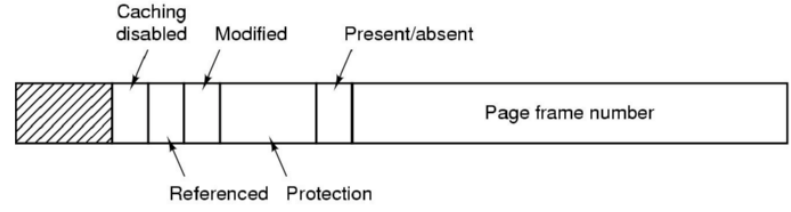
\includegraphics[width=12cm,height=2.7cm,keepaspectratio]{ch9_10.png}}
				\end{figure}
				\\Poiché la Page Table è troppo grande per essere nella CPU, viene memorizzata in RAM. Nella CPU sono invece presenti due registri:
				\begin{itemize}
					\item \textbf{Page-Table Base Register} (\textbf{PTBR}): indirizzo base della Page Table in RAM;
					\item \textbf{Page-Table Length Register} (\textbf{PTLR}): dimensione della Page Table;
				\end{itemize}
				Notare che l'utilizzo di questa tecnica richiede due accessi a memoria per accedere all'istruzione/dato (uno per tradurre indirizzo logico in fisico e uno per eseguire l'operazione). Questo dimezza la velocità della memoria. Per risolvere questo problema può essere usata una cache ad accesso diretto (CAM o Memoria Associativa) detta \textbf{Translaction Lookaside Buffers} (\textbf{TLB}). La memoria associativa è progettata in modo che si possa effettuare ricerca in parallelo su tutte le entry e solo la entry che matcha (se presente e massimo una) produce l'output desiderato. Essendo una cache può esserci \textit{TLB miss} ma comunque migliora le prestazioni. 
				\begin{figure}[ht!]
					\centering{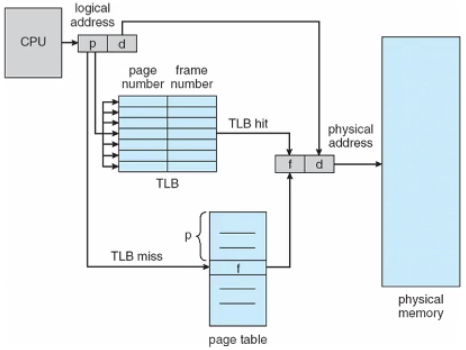
\includegraphics[width=12cm,height=5cm,keepaspectratio]{ch9_12.png}}
				\end{figure}
				\newpage
				\noindent La TLB è solitamente piccola, da 64 a 1024 entry.
				\begin{figure}[ht!]
					\centering{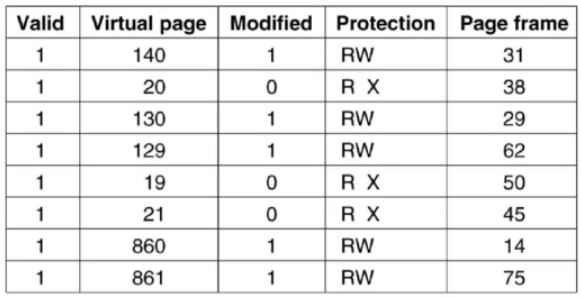
\includegraphics[width=12cm,height=4cm,keepaspectratio]{ch9_11.png}}
				\end{figure}
				\\Vediamo come può essere calcolato l'\textbf{Effective Access Time} (\textbf{EAT}): ipotizziamo di avere un \textit{hit ratio} dell'80\% e che il tempo di accesso alla memoria in caso di \textit{TLB hit} sia di 10 ns (quindi di 20 ns in caso di miss):
				\begin{itemize}
					\item EAT = 0.8 * 10 + 0.2 * 20 = 12 ns
				\end{itemize}

			\subsubsection{Protezione}
				In un ambiente paginato, la protezione della memoria è assicurata dai \textbf{bit di protezione} associati a ogni frame; normalmente tali bit si trovano nella tabella delle pagine (e nella TLB) e sono usati, ad esempio, per determinare se una pagina si può leggere e scrivere oppure soltanto leggere. 
				\\Quando si interroga la page table per calcolare l’indirizzo fisico, vengono controllati i bit di protezione per verificare che non si scriva in una pagina di sola lettura. Un tale tentativo causerebbe la generazione di un’eccezione hardware per il SO. Questo metodo si può facilmente estendere per fornire un livello di protezione più perfezionato aggiungendo bit.
				\\Di solito si associa a ciascun elemento della tabella delle pagine un ulteriore bit, detto \textbf{bit di validità}. Tale bit, impostato a valido, indica che la pagina corrispondente è nello spazio d’indirizzi logici del processo, quindi è una pagina valida. Il bit di validità consente quindi di riconoscere gli indirizzi illegali e di notificarne la presenza attraverso un’eccezione.
				\newpage
				\noindent Per esempio, supponiamo che in un sistema con uno spazio di indirizzi di 14 bit (da 0 a 16.383) si abbia un programma che deve usare soltanto gli indirizzi da 0 a 10.468 e che le pagine sono di 2 kB.
				\begin{figure}[ht!]
					\centering{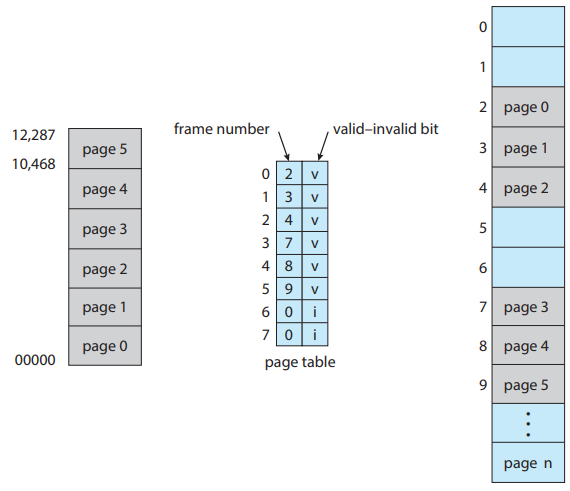
\includegraphics[width=12cm,height=6.5cm,keepaspectratio]{ch9_13.png}}
				\end{figure}
				\\Gli indirizzi nelle pagine 0, 1, 2, 3, 4 e 5 sono tradotti normalmente tramite la tabella delle pagine. D’altra parte, ogni tentativo di generare un indirizzo nelle pagine 6 o 7 trova il bit di validità non valido; in questo caso il calcolatore invia un’eccezione al sistema operativo (riferimento di pagina non valido).
				\\Questo schema ha creato un problema: poiché il programma si estende solo fino all’indirizzo 10.468, ogni riferimento oltre tale indirizzo è illegale; i riferimenti alla pagina 5 sono tuttavia classificati come validi, e ciò rende validi gli accessi sino all’indirizzo 12.287; solo gli indirizzi da 12.288 a 16.383 sono non validi. Tale problema è dovuto alla dimensione delle pagine di 2 kb e corrisponde alla frammentazione interna della paginazione.
			
			\subsubsection{Pagine Condivise}
				Un altro vantaggio della paginazione consiste nella possibilità di condividere pagine  tra processi, con conseguente risparmio di RAM.
				\\Se una pagina di codice (es. funzione di libreria) deve essere condivisa, deve contenere \textbf{codice rientrante}. Il codice rientrante non cambia durante l’esecuzione. Quindi, due o più processi possono eseguirlo nello stesso momento. I dati usati da queste funzioni sono invece tipicamente privati.
				\\Si consideri un sistema con 40 utenti, ciascuno dei quali usa un text editor. Se tale programma è formato da 150 kb di codice e 50 kB di spazio di dati, per gestire i 40 utenti sono necessari 8000 kB. Se invece il codice viene condiviso sono necessari solo 2150 kB.
				\newpage
				\begin{figure}[ht!]
					\centering{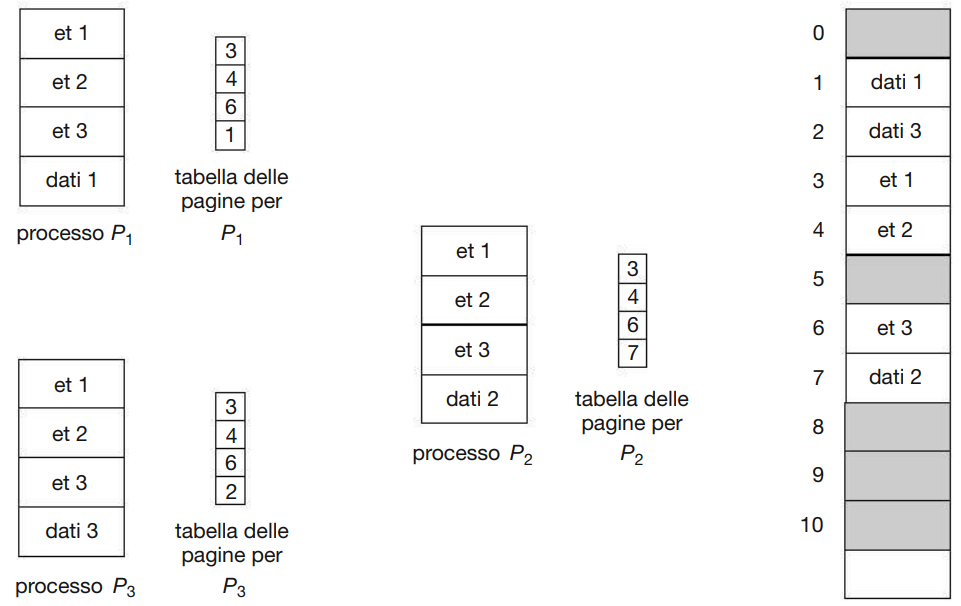
\includegraphics[width=12cm,height=6.5cm,keepaspectratio]{ch9_14.png}}
				\end{figure}
				\noindent Il codice condiviso è read-only ma possono essere condivise anche pagine di dati read/write per permettere la comunicazione tra processi.

		\subsection{Struttura della Page Table}
			La tabella delle pagine potrebbe diventare enorme. Considerariamo ad esempio uno spazio di indirizzamento logico a 32 bit e pagine di 4kB. La tabella delle pagine dovrebbe avere circa 1 milione di entry ($2^{32}/2^{12}$) e, se ogni entry è di 4 B, ogni processo occuperebbe 4 MB di memoria fisica solo per essa. Inoltre, bisogna notare che la memoria occupata dovrebbe essere contigua perché la tabella viene usata come un array ad accesso diretto.
			\\Quello che vogliamo fare è  eliminare il problema della contiguità della memoria. Vediamo alcune delle tecniche più comuni usate per strutturare la tabella delle pagine:
			\begin{itemize}
				\item \textbf{paginazione gerarchica};
				\item \textbf{hashed page table};
				\item \textbf{inverted page table}.
			\end{itemize}

			\newpage
			\subsubsection{Paginazione Gerarchica}
				La paginazione gerarchica è una soluzione semplice per evitare di collocare la page table in modo contiguo in RAM. Questo metodo consiste nell’adottare un algoritmo di paginazione a più livelli, in cui la tabella stessa è paginata. 
				\begin{figure}[ht!]
					\centering{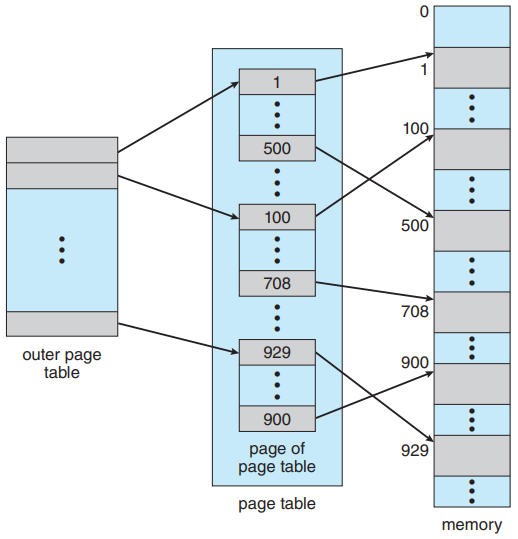
\includegraphics[width=12cm,height=6cm,keepaspectratio]{ch9_15.png}}
				\end{figure}
				\\Si consideri l'esempio di macchina a 32 bit con dimensione delle pagine di 4 kB ed entry nella page table di 4 byte. Ciascun indirizzo logico è suddiviso in un numero di pagina di 20 bit e in un offset di pagina di 12. Paginando la tabella delle pagine (4 MB in pagine da 4 kB), anche il numero di pagina è suddiviso in un numero di pagina di 10 bit e un offset di 10 (una entry occupa 4 byte, quindi non c'è bisogno di accedere a ogni byte ma ad uno ogni 4).
				\begin{figure}[ht!]
					\centering{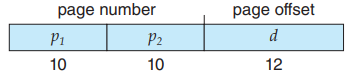
\includegraphics[width=12cm,height=1.2 cm,keepaspectratio]{ch9_16.png}}
				\end{figure}
				\\Poiché la traduzione degli indirizzi si svolge dalla tabella esterna delle pagine verso l’interno, questo metodo è anche noto come \textbf{tabella delle pagine ad associazione diretta} (\textbf{forward-mapped page table}).
				\\Tra gli svantaggi che possiamo notare c'è la maggiore occupazione di memoria (overhead) e il dover effettuare un ulteriori accessi all a RAM.
				\\La paginazione a due livelli non è adatta per sistemi con uno spazio di indirizzi logici a 64 bit. Si supponga che la dimensione delle pagine di questo sistema sia di 4 kB. In questo caso, la tabella delle pagine conterrà fino a $2^{52}$ elementi. Adottando uno schema di paginazione a due livelli, le page table interne possono occupare una pagina, o contenere $2^{10}$ elementi di 4 byte. 
				\begin{figure}[ht!]
					\centering{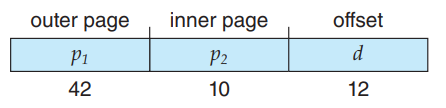
\includegraphics[width=12cm,height=1.3cm,keepaspectratio]{ch9_17.png}}
				\end{figure}
				\\La page table esterna è di $2^{42}$ elementi. La soluzione per evitare una tabella tanto grande consiste nel suddividerla in parti più piccole. Per esempio, si può paginare ottenendo uno schema di paginazione a tre livelli. Si supponga che la tabella esterna delle pagine sia costituita di pagine di dimensione ordinaria ($2^{10}$ elementi, o $2^{12}$ byte); uno spazio d’indirizzi a 64 bit è ancora enorme:
				\begin{figure}[ht!]
					\centering{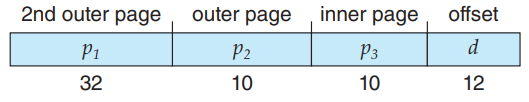
\includegraphics[width=12cm,height=1.3cm,keepaspectratio]{ch9_18.png}}
				\end{figure}
				\\Il passo successivo sarebbe uno schema di paginazione a quattro livelli, in cui si pagina anche la tabella esterna di secondo livello delle pagine, e così via.

			\subsubsection{Hashed Page Table}
				Un metodo per gestire spazi d’indirizzi oltre i 32 bit consiste nell’impiego di una hash table, in cui l’argomento della funzione hash è il numero della pagina virtuale. Ogni elemento della tabella contiene una lista concatenata di elementi che la funzione di hash fa corrispondere alla stessa locazione ed è composto da tre campi: (1) numero della pagina virtuale, (2) indirizzo del frame corrispondente alla pagina virtuale e (3) puntatore al successivo elemento della lista.
				\\Algoritmo: si applica la funzione hash al numero della pagina virtuale contenuto nell’indirizzo virtuale, identificando un elemento della tabella. Si confronta il numero di pagina virtuale con il campo (1) del primo elemento della lista concatenata: se i valori coincidono, si usa il campo 2 per generare l’indirizzo fisico altrimenti, vengono esaminati gli elementi successivi.
				\begin{figure}[ht!]
					\centering{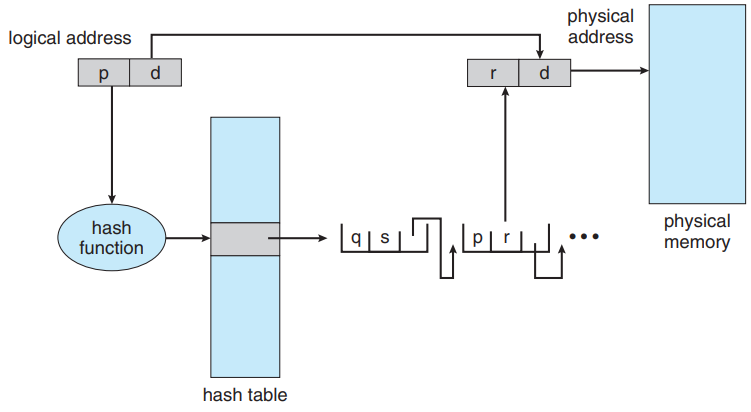
\includegraphics[width=12cm,height=5cm,keepaspectratio]{ch9_19.png}}
				\end{figure}
				\\Per questo schema è stata proposta una variante: la \textbf{page table a gruppi} (\textbf{clustered page table}), simile alla hash page table ma ciascun elemento della hash table contiene i riferimenti alle pagine fisiche corrispondenti a un gruppo di pagine virtuali contigue (per esempio 16). Queste tabelle sono particolarmente utili per gli spazi d’indirizzi sparsi, in cui i riferimenti alla memoria non sono contigui.

			\subsubsection{Inverted Page Table}
				Generalmente, si associa una tabella delle pagine a ogni processo e tale tabella contiene un elemento per ogni pagina virtuale che il processo sta usando. Uno degli inconvenienti di questo metodo è che ciascuna page table può occupare grandi quantità di memoria fisica.
				\\Per risolvere questo problema si può fare uso della tabella delle pagine invertita. Una inverted page table ha un elemento per ogni frame. Ciascun elemento è costituito dell’indirizzo virtuale della pagina memorizzata in quella reale locazione di memoria (\textit{p}) e dal \textit{pid} del processo che possiede tale pagina (perché processi diversi possono usare lo stesso \textit{p}). Quindi, nel sistema esiste una sola tabella delle pagine che ha un solo elemento per ciascuna pagina di memoria fisica. Se avviene il match con l'\textit{i-esima} entri, \textit{i} corrisponde all'indirizzo fisico.
				\begin{figure}[ht!]
					\centering{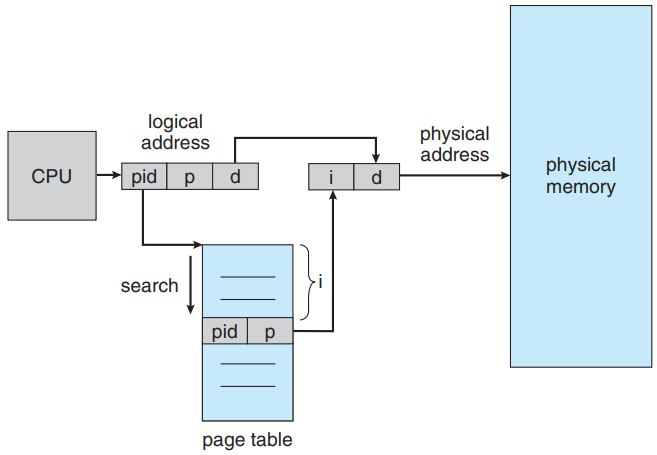
\includegraphics[width=12cm,height=5cm,keepaspectratio]{ch9_20.png}}
				\end{figure}
				\\I vantaggi di questa tecnica sono che la page table ha dimensione minori (dipenda dal numero di frame, non dalla dimensione dello spazio di indirizzamenti virtuale) e che c'è una unica tabella per tutti i processi (ogni frame è associato a un solo processo). Lo svantaggio è che non si ha accesso diretto (serve ricerca) e questo causa rallentamenti. Per eliminare questo problema le IPT sono associate a tabelle di hash.
				\begin{figure}[ht!]
					\centering{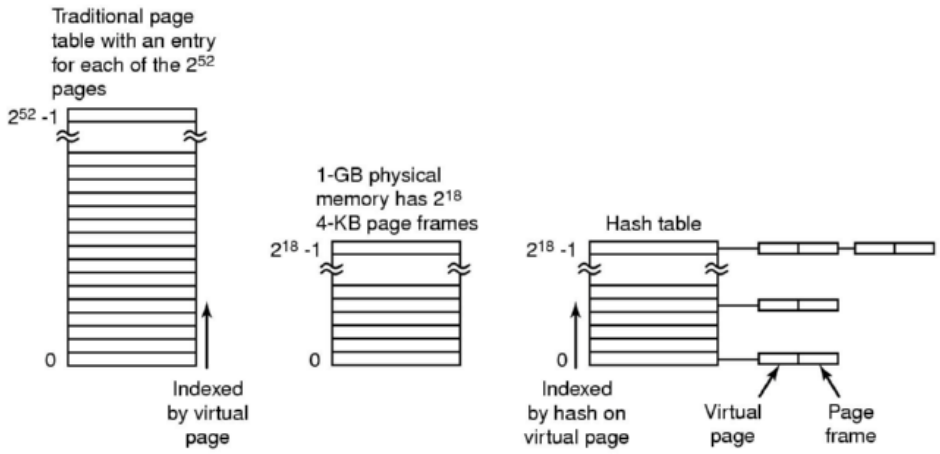
\includegraphics[width=12cm,height=5cm,keepaspectratio]{ch9_21.png}}
				\end{figure}
				
		\subsection{Swapping}
			Per essere eseguito, un processo deve trovarsi in RAM. Tuttavia, può essere temporaneamente tolto da essa (\textbf{swap/roll out}), essere spostato in una memoria ausiliaria (\textbf{backing store}) e in seguito riportato in memoria per continuare (\textbf{swap/roll in}) l’esecuzione. Questo procedimento si chiama avvicendamento dei processi in memoria (swapping). Grazie allo swapping lo spazio degli indirizzi fisici di tutti i processi può eccedere la reale dimensione della memoria fisica del sistema, aumentando il grado di multiprogrammazione possibile.
			\begin{figure}[ht!]
				\centering{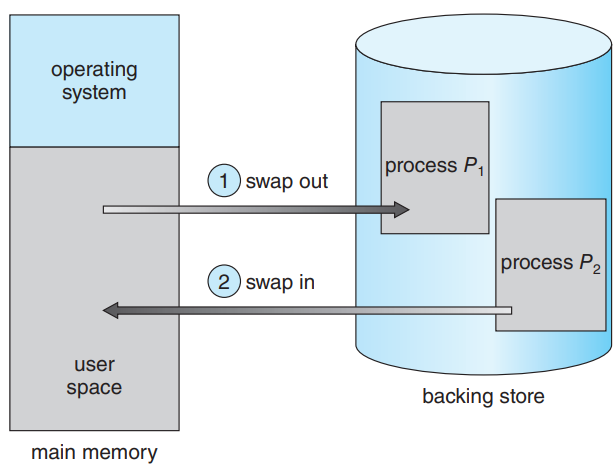
\includegraphics[width=12cm,height=5cm,keepaspectratio]{ch9_22.png}}
			\end{figure}

			\subsubsection{Standard Swapping}
				L’avvicendamento standard riguarda lo spostamento dei processi tra la RAM e backing store, di solito costituita da un disco veloce. Tale memoria deve essere abbastanza ampia da contenere le copie di tutte le immagini di memoria di tutti i processi utenti, e deve permettere un accesso diretto ad esse. Il sistema mantiene una coda dei processi pronti (\textit{ready queue}) formata dai processi pronti per l’esecuzione. Quando lo scheduler decide di eseguire un processo, richiama il dispatcher, che controlla se il primo processo della coda si trova in memoria centrale. Se non c'è, e in questa non c’è spazio libero, il dispatcher scarica un processo dalla memoria e vi carica il processo richiesto dallo scheduler, quindi ricarica i registri e trasferisce il controllo al processo selezionato.
				\\In un tale sistema d’avvicendamento, il tempo di context-switching è piuttosto elevato. Si pensi a un processo di 100 MB e a una memoria ausiliaria costituita da un normale hard disk con velocità di trasferimento di 50 MB al secondo. Il trasferimento del processo richiede: 100 MB / 50 MB al secondo = 2 secondi. Dal momento che dobbiamo scaricare e poi ricaricare il processo, il tempo totale è di circa 4 s.
				\\Occorre notare che la maggior parte del tempo d’avvicendamento è data dal tempo di trasferimento e che questo è direttamente proporzionale alla quantità di memoria trasferita. Perciò sarebbe utile sapere quanta memoria sia effettivamente usata da un processo e non solo quanta questo potrebbe usarne, poiché in questo caso è necessario trasferire solo quanto è effettivamente utilizzato, riducendo il tempo d’avvicendamento (\textbf{swapping con paging}). 
				\\Per scaricare un processo dalla memoria è necessario essere certi che sia completamente inattivo. Particolare importanza ha l’attesa di I/O: quando decidiamo di scaricare un processo per liberare la memoria, tale processo può essere nell’attesa del completamento di un’operazione di I/O. Tuttavia, se un dispositivo di I/O accede in modo asincrono alle aree di I/O della memoria (buffer) utente, il processo non può essere scaricato. Si supponga che l’operazione di I/O sia stata accodata, perché il dispositivo era occupato. Se il processo P2 s’avvicendasse al processo P1, l’operazione di I/O potrebbe tentare di usare la memoria che attualmente appartiene al processo P2. Questo problema si può risolvere in due modi: non scaricando dalla memoria un processo con operazioni di I/O pendenti, oppure eseguendo operazioni di I/O solo in buffer del SO. Trasferimenti fra tali aree del sistema operativo e la memoria assegnata al processo possono poi avvenire solo quando il processo è presente in RAM. Si noti che questo meccanismo di memorizzazione (\textbf{double buffering}) aggiunge overhead. Abbiamo infatti bisogno di copiare nuovamente i dati, dalla memoria del kernel alla memoria utente, prima che il processo utente possa accedervi.
				\\Attualmente l’avvicendamento nella sua forma standard si usa in pochi sistemi; richiede infatti un elevato tempo di trasferimento, e consente un tempo di esecuzione troppo breve per essere considerato una soluzione ragionevole al problema di gestione della memoria.

			\subsubsection{Swapping in Sistemi Mobili}
				Mentre la maggior parte dei SO per PC e server supporta qualche versione di swapping, i sistemi mobili in genere non ne supportano. Questi utilizzano solitamente, come memoria di massa, la memoria flash al posto dei dischi rigidi, più voluminosi. Il vincolo che ne deriva in termini di spazio è una delle ragioni per cui si evitalo swapping dei processi. Inoltre, vi sono il numero limitato di scritture che una memoria flash può sopportare prima di diventare inaffidabile e il trasferimento tra memoria centrale e memoria flash è lento.
				\\Invece di usare lo swapping, se la memoria disponibile scende al di sotto di una certa soglia, iOS di Apple chiede alle applicazioni di rinunciare volontariamente alla memoria allocata. I dati di sola lettura vengono rimossi dal sistema e successivamente ricaricati dalla memoria flash, se necessario. I dati che sono stati modificati (per esempio lo stack) non vengono rimossi. Tuttavia, tutte le applicazioni che non riescono a liberare memoria a sufficienza possono essere terminate dal SO.
				\\Android non supporta l’avvicendamento e adotta una strategia simile a quella di iOS. Anche Android può terminare un processo qualora la memoria libera disponibile non sia sufficiente. Tuttavia, prima di terminarlo, scrive lo stato dell’applicazione nella memoria flash, in modo che il processo possa essere rapidamente riavviato.

	\section{Memoria Virtuale}
		
		\subsection{Introduzione}
			Nel precedente capitolo sono state esaminate varie strategie di gestione della memoria. Hanno tutte lo stesso scopo: tenere contemporaneamente più processi in memoria per permettere la multiprogrammazione; tuttavia esse tendono a richiedere che l’intero processo si trovi in memoria prima di essere eseguito.
			\\La \textbf{memoria virtuale}, definisce una separazione tra gli indirizzi logici e fisici e solo una parte degli indirizzi logici sono mappati in quelli fisici (non viene caricato tutto il programma in RAM). Il vantaggio principale di questa tecnica è quello di permettere che i programmi siano più grandi della memoria fisica; inoltre la memoria virtuale astrae la memoria centrale in un vettore di memorizzazione molto grande e uniforme, separando la memoria logica, com’è vista dall’utente, da quella fisica. Questa tecnica libera i programmatori dai problemi di limitazione della memoria. Inoltre, permette l'esecuzione di più programi, ai processi di condividere facilmente file e di realizzare memorie condivise, e fornisce un meccanismo efficiente per la creazione dei processi. La memoria virtuale è però difficile da realizzare e, s’è usata scorrettamente, può ridurre di molto le prestazioni del sistema. 
			\begin{figure}[ht!]
				\centering{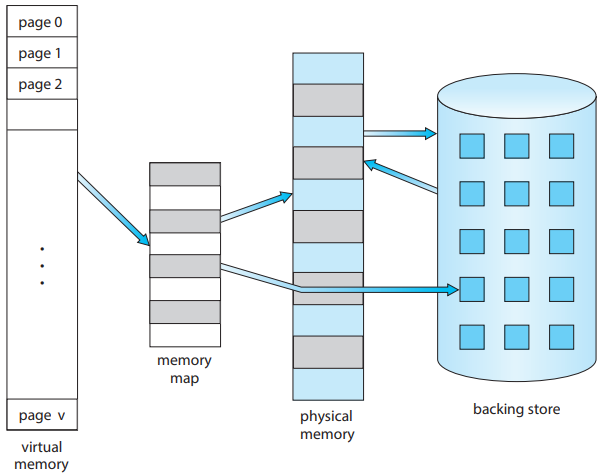
\includegraphics[width=12cm,height=4cm,keepaspectratio]{ch9_23.png}}
			\end{figure}
			\\L’espressione \textbf{spazio degli indirizzi virtuali} si riferisce alla collocazione dei processi in memoria dal punto di vista logico (o virtuale). Tipicamente, da tale punto di vista, un processo inizia in corrispondenza di un certo indirizzo logico (es. l’indirizzo 0) e si estende in uno spazio di memoria contigua.
			\begin{figure}[ht!]
				\centering{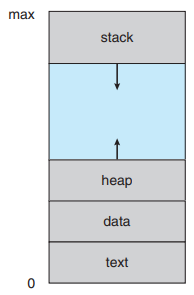
\includegraphics[width=12cm,height=3.5cm,keepaspectratio]{ch9_24.png}}
			\end{figure}
			\newpage
			\noindent Come si ricorderà, è tuttavia possibile organizzare la memoria fisica in frame di pagine; in questo caso i frame delle pagine fisiche assegnati ai processi possono non essere contigui. Spetta alla MMU associare le pagine logiche a quelle fisiche.
			\\Si noti come allo heap sia lasciato spazio per crescere verso l’alto nello spazio di memoria, poiché esso ospita la memoria allocata dinamicamente. In modo analogo, consentiamo allo stack di svilupparsi verso il basso quando vengono effettuate ripetute chiamate di funzione. Lo spazio vuoto (o buco) che separa lo heap dallo stack è parte dello spazio degli indirizzi virtuali, ma richiede pagine fisiche reali solo nel caso che lo heap o lo stack crescano. Uno spazio degli indirizzi virtuali che contiene buchi si definisce \textbf{sparso}. Un simile
			spazio degli indirizzi è utile, poiché i buchi possono essere riempiti grazie all’espansione dei segmenti heap o stack, oppure se vogliamo collegare dinamicamente delle
			librerie (o altri oggetti condivisi) durante l’esecuzione del programma.
			\\Oltre a separare la memoria logica da quella fisica, la memoria virtuale offre il vantaggio di condividere i file e la memoria fra duo o più processi, mediante la condivisione delle pagine. 
			\begin{figure}[ht!]
				\centering{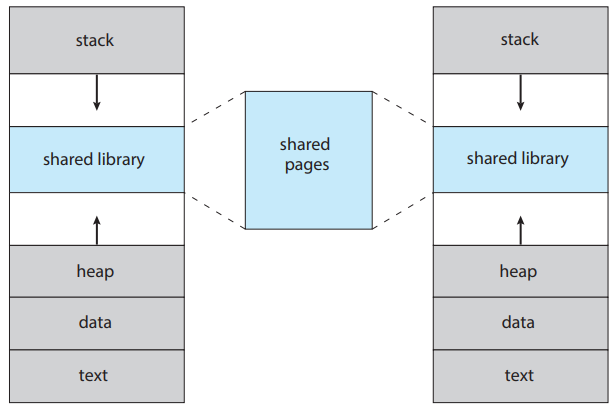
\includegraphics[width=12cm,height=4cm,keepaspectratio]{ch9_25.png}}
			\end{figure}
			\\Ciò comporta i seguenti vantaggi:
			\begin{itemize}
				\item le librerie di sistema sono condivisibili da diversi processi associando (“mappando”) l’oggetto di memoria condiviso a uno spazio degli indirizzi virtuali. Benché ciascun processo veda le librerie condivise come parte del proprio spazio degli indirizzi virtuali, le pagine che ospitano effettivamente le librerie nella memoria fisica sono in condivisione tra tutti i processi. In genere le librerie si associano allo spazio di ogni processo a loro collegato, in modalità di sola lettura;
			   \item in maniera analoga, la memoria può essere condivisa tra processi distinti. Due o più processi possono comunicare condividendo memoria. La memoria virtuale permette a un processo di creare una regione di memoria condivisibile da un altro processo. I processi che condividono questa regione la considerano parte del proprio spazio degli indirizzi virtuali, malgrado le pagine fisiche siano, in realtà, condivise;
			   \item Le pagine possono essere condivise durante la creazione di un processo mediante la chiamata di sistema \textit{fork()}, così da velocizzare la generazione dei processi.
			\end{itemize}

		\subsection{Paginazione su Richiesta (Demand Paging)}

			La \textbf{paginazione su richiesta} è una tecnica che consiste nel caricare le pagine nel momento in cui servono realmente e che viene comunemente adottata dai sistemi con memoria virtuale. Un sistema di paginazione su richiesta è simile a un sistema paginato con avvicendamento dei processi in memoria (swapping). I processi risiedono in memoria secondaria e per eseguirli occorre caricarli in memoria. Tuttavia, anziché caricare l’intero processo, si esegue un avvicendamento “pigro” (\textbf{lazy swapping}): non si carica mai in memoria una pagina che non sia necessaria. Nell’ambito dei sistemi con paginazione su richiesta l’uso del termine "swapping" non è appropriato: uno swapper manipola interi processi mentre un \textbf{paginatore} (pager) gestisce le singole pagine dei processi.

			\subsubsection{Concetti Fondamentali}
				Quando un processo sta per essere caricato in memoria, il paginatore ipotizza quali pagine saranno usate prima che il processo sia nuovamente scaricato dalla memoria (swap in) e trasferisce in memoria (swap out) solo quest pagine. 
				\\Con tale schema è necessario che l’hardware fornisca un meccanismo che distingue le pagine presenti in memoria da quelle nei dischi. A tal fine è utilizzabile un \textbf{bit di validità}: impostato come “valido” se la pagina corrispondente è valida ed è presente in memoria e come “non valido” se la pagina non è valida (cioè non appartiene allo spazio d’indirizzi logici del processo) oppure è valida ma è attualmente nel disco. L’elemento della tabella delle pagine di una pagina caricata in memoria s’imposta come al solito, mentre l’elemento della tabella delle pagine corrispondente a una pagina che attualmente non è in memoria è semplicemente contrassegnato come non valido oppure contiene l’indirizzo della pagina su disco.
				\begin{figure}[ht!]
					\centering{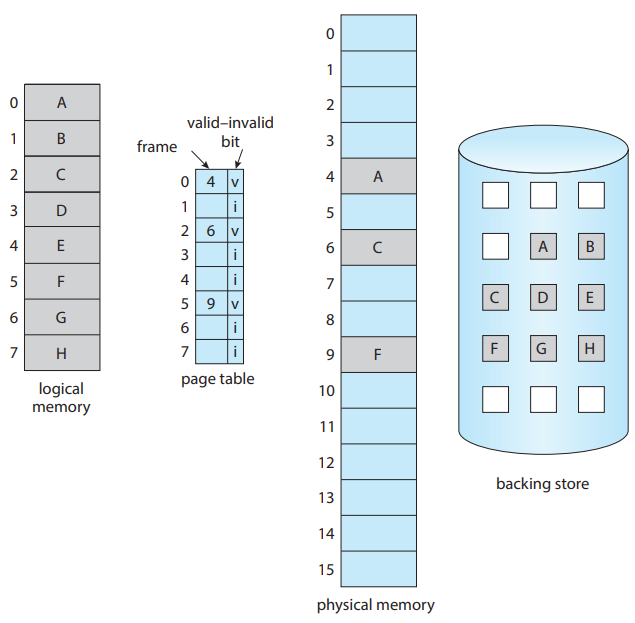
\includegraphics[width=12cm,height=6.1cm,keepaspectratio]{ch9_26.png}}
				\end{figure}
				\\Occorre notare che indicare una pagina come non valida non sortisce alcun effetto se il processo non tenta mai di accedervi. Quindi, se l’ipotesi del paginatore è esatta e si caricano tutte e solo le pagine che servono  effettivamente, il processo è eseguito proprio come se fossero state caricate tutte le pagine. Durante  l’esecuzione, finchè il processo accede alle pagine \textbf{residenti in memoria}, l’esecuzione procede come di consueto.
				\\L’accesso a una pagina contrassegnata come non valida causa un evento o eccezione di \textbf{page fault}. L’hardware di paginazione, traducendo l’indirizzo attraverso la tabella delle pagine, nota che il bit è non valido e genera una trap per il SO. La procedura di gestione dell’eccezione di page fault è la seguente:
				\begin{figure}[ht!]
					\centering{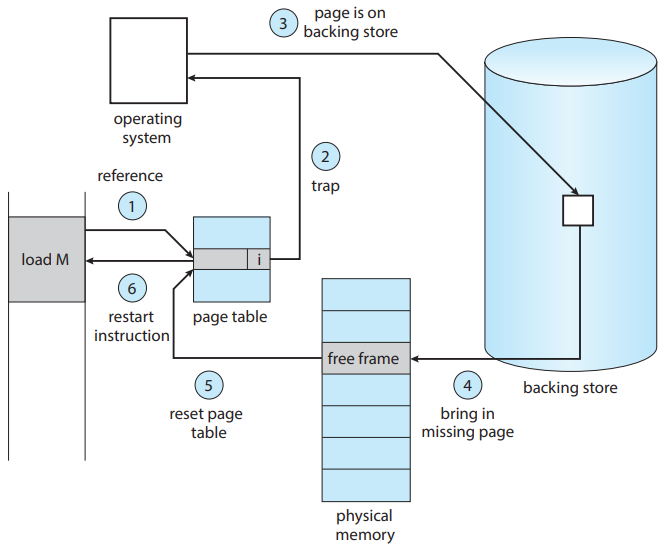
\includegraphics[width=12cm,height=6.5cm,keepaspectratio]{ch9_27.png}}
				\end{figure}
				\begin{enumerate}
					\item si controlla una tabella interna per il processo per stabilire se il riferimento fosse un accesso alla memoria valido o non valido;
					\item se il riferimento non era valido, si termina il processo. Se era un riferimento valido, ma la pagina non era ancora stata portata in memoria, se ne effettua il caricamento;
					\item si individua un frame libero, per esempio prelevandone uno dalla lista dei frame liberi;
					\item si programma un’operazione sui dischi per trasferire la pagina desiderata nel frame appena assegnato;
					\item quando la lettura dal disco è completata, si modificano la tabella interna, conservata con il processo, e la tabella delle pagine per indicare che la pagina si trova attualmente in memoria (bi di validità = 'v');
					\item si riavvia l’istruzione interrotta dall’eccezione. A questo punto il processo può
					accedere alla pagina come se questa fosse stata sempre presente in memoria.
				\end{enumerate}
				Il caso estremo, è l'avvio di un processo senza pagine in memoria. Quando il SO carica nel PC l’indirizzo della prima istruzione del processo, il processo genera immediatamente un page fault. Una volta portata la pagina in memoria, il processo continua l’esecuzione, generando page fault fino a che tutte le pagine necessarie non si trovino effettivamente in memoria; a questo punto si può eseguire il processo senza ulteriori richieste. Lo schema descritto è una \textbf{paginazione su richiesta pura} (una pagina non si trasferisce mai in memoria se non viene richiesta).
				\\In teoria alcuni programmi possono accedere a diverse nuove pagine all’esecuzione di ogni istruzione (una pagina per l’istruzione e molte per i dati), eventualmente causando più page fault. In un caso simile le prestazioni del sistema sarebbero inaccettabili. Fortunatamente l’analisi dei programmi in esecuzione mostra che questo comportamento è estremamente improbabile perché i programmi tendono ad avere una \textbf{località dei riferimenti}.
				\\L’hardware di supporto alla paginazione su richiesta è lo stesso che è richiesto per la paginazione e l’avvicendamento dei processi in memoria:
				\begin{itemize}
					\item \textbf{tabella delle pagine}: ha la capacità di contrassegnare un elemento come non valido attraverso un bit di validità oppure un valore speciale dei bit di protezione;
					\item \textbf{memoria secondaria}: conserva le pagine non presenti in memoria centrale. Generalmente la memoria secondaria è costituita da un disco ad alta velocità detto dispositivo di swap; la sezione del disco usata a questo scopo si chiama \textbf{area di avvicendamento} (\textbf{swap space}).
				\end{itemize}
				Uno dei requisiti cruciali del Demand paging è la possibilità di rieseguire un'istruzione dopo un page fault. Avendo salvato lo stato del processo interrotto (registri, PC\dots) al momento del page fault, occorrerà riavviare il processo esattamente dallo stesso punto e con lo stesso stato, eccezion fatta per la presenza della pagina desiderata in memoria. Nella maggior parte dei casi questo requisito è facile da soddisfare. Un page fault si può verificare per qualsiasi riferimento alla memoria. Se si verifica durante la fase di fetch (prelievo) di un’istruzione, l’esecuzione si può riavviare effettuando nuovamente il fetch. Se si verifica durante il fetch di un operando, bisogna effettuare nuovamente fetch e decode dell’istruzione, quindi si può prelevare l’operando. Come caso limite si consideri un’istruzione a tre indirizzi, per esempio la somma (ADD) del contenuto di A al contenuto di B, con risultato posto in C. I passi necessari per eseguire l’istruzione sono i seguenti:
				\begin{enumerate}
					\item fetch e decodifica dell’istruzione (ADD);
					\item prelievo del contenuto di A;
					\item prelievo del contenuto di B;
					\item addizione del contenuto di A al contenuto di B
					\item memorizzazione della somma in C.
				\end{enumerate}
				Se il page fault avviene al momento della memorizzazione in C, poiché C si trova in una pagina che non è in memoria, occorre prelevare la pagina desiderata, caricarla in memoria, correggere la tabella delle pagine e riavviare l’istruzione. Il riavvio dell’istruzione richiede una nuova operazione di fetch, con nuova decodifica e nuovo prelievo dei due operandi; infine occorre ripetere l’addizione.

			\subsubsection{Free-Frame List}
				Quando si verifica un page fault, il SO deve trovare un frame libero dove allocare la pagina. Perché questa ricerca sia rapida, viene utililzzata una lista dei frame liberi (\textbf{free-frame list}).
				\begin{figure}[ht!]
					\centering{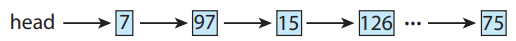
\includegraphics[width=12cm,height=0.7cm,keepaspectratio]{ch9_28.png}}
				\end{figure}
				\\I SO solitamente allocano i frame liberi usando una tecnica conosciuta come \textbf{zero-fill-on-demand}, ovvero i frame vengono riempiti di zeri prima di essere allocati.
				\\Quando il sistema viene avviato, tutta la memoria disponibile appartiene alla free-frame list.

			\subsubsection{Prestazioni del Demand Paging}
				La paginazione su richiesta può avere un effetto rilevante sulle prestazioni. Il motivo si può comprendere calcolando il tempo d’accesso effettivo per una memoria con paginazione su richiesta. Attualmente, nella maggior parte dei calcolatori il tempo d’accesso alla memoria varia da 10 a 200 nanosecondi. Finché non si verifichino page fault, il tempo d’accesso effettivo è uguale al tempo d’accesso alla memoria. Se però si verifica un page fault, occorre prima leggere dal disco la pagina interessata e quindi accedere alla parola della memoria desiderata.
				\\Supponendo che \textit{p} sia la probabilità che si verifichi un page fault (0 $<=$ p $<=$ 1), è probabile che \textit{p} sia molto vicina allo zero, cioè che ci siano solo pochi fault. Il tempo d’accesso effettivo è dato da:
				\begin{center}
					\textit{tempo d’accesso effettivo = (1 – p) – ma + p × tempo di gestione del page fault}
				\end{center}
				Per calcolare il tempo d’accesso effettivo occorre conoscere il tempo necessario alla gestione di un page fault. In tal caso si deve eseguire la seguente sequenza:
				\begin{enumerate}
					\item trap per il sistema operativo;
					\item salvataggio dei registri utente e dello stato del processo;
					\item verifica che l’interruzione sia dovuta o meno a un page fault;
					\item . controllo della correttezza del riferimento alla pagina e determinazione della locazione della pagina nel disco;
					\item lettura dal disco e trasferimento in un frame libero:
					\begin{enumerate}
						\item attesa nella coda relativa a questo dispositivo finché la richiesta di lettura non sia servita;
						\item attesa del tempo di posizionamento e latenza del dispositivo;
						\item inizio del trasferimento della pagina in un frame libero;
					\end{enumerate}
					\item durante l’attesa, allocazione della CPU a un altro processo utente (scheduling della CPU, facoltativo);
					\item ricezione di un’interruzione dal controllore del disco (I/O completato);
					\item salvataggio dei registri e dello stato dell’altro processo utente (se è stato eseguito il passo 6);
					\item verifica della provenienza dell’interruzione dal disco;
					\item aggiornamento della tabella delle pagine e di altre tabelle per segnalare che la pagina richiesta è attualmente presente in memoria;
					\item attesa che la CPU sia nuovamente assegnata a questo processo;
					\item ripristino dei registri utente, dello stato del processo e della nuova tabella delle pagine, quindi ripresa dell’istruzione interrotta.
				\end{enumerate}
				Non sempre sono necessari tutti i passi sopra elencati. Nel passo 6, per esempio, si ipotizza che la CPU sia assegnata a un altro processo durante un’operazione di I/O. Tale possibilità permette la multiprogrammazione per mantenere occupata la CPU, ma una volta completato il trasferimento di I/o implica un dispendio di tempo per riprendere la procedura di servizio dell’eccezione di page fault.
				\\In ogni caso, il tempo di servizio dell’eccezione di page fault ha tre componenti:
				\begin{itemize}
					\item servizio del segnale di eccezione di page fault;
					\item lettura della pagina da disco;
					\item riavvio del processo.
				\end{itemize}
				La prima e la terza operazione si possono ridurre, per mezzo di un’accurata codifica, ad alcune centinaia di istruzioni. Ciascuna di queste operazioni può quindi richiedere da 1 a 100 microsecondi. D’altra parte, il tempo di trasferimento di pagina è probabilmente vicino a 8 ms (un disco ha in genere un tempo di latenza di 3 ms, un tempo di posizionamento di 5 ms e un tempo di trasferimento di 0,05 ms, quindi il tempo totale della paginazione è dell’ordine di 8 ms, comprendendo le tempistiche hardware e software). Inoltre nel calcolo si è considerato solo il tempo di servizio del dispositivo. Se una coda di processi è in attesa del dispositivo è necessario considerare anche il tempo di accodamento del dispositivo, poiché occorre attendere che il dispositivo di paginazione sia libero per servire la richiesta, quindi il tempo di trasferimento aumenta ulteriormente.
				\newpage
				\noindent Considerando un tempo medio di servizio dell’eccezione di page fault di 8 ms e un tempo d’accesso alla memoria di 200 ns, il \textbf{tempo effettivo d’accesso} (\textbf{EAT}) in ns è il seguente:
				\begin{figure}[ht!]
					\centering{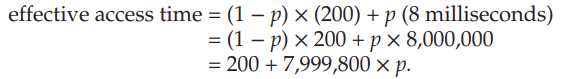
\includegraphics[width=12cm,height=1.2cm,keepaspectratio]{ch9_29.png}}
				\end{figure}
				\\Il tempo d’accesso effettivo è direttamente proporzionale al tasso di page fault (\textbf{page-fault rate}). Se un accesso su 1000 accusa un page fault, il tempo d’accesso effettivo è di 8,2 microsecondi. Impiegando la paginazione su richiesta, il calcolatore è
				rallentato di un fattore pari a 40! Se si desidera un rallentamento inferiore al 10 per cento, occorre contenere la probabilità di page fault al seguente livello:
				\begin{figure}[ht!]
					\centering{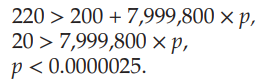
\includegraphics[width=12cm,height=1.3cm,keepaspectratio]{ch9_30.png}}
				\end{figure}
				\\Quindi, per mantenere a un livello ragionevole il rallentamento dovuto alla paginazione, si può permettere meno di un page fault ogni 399.990 accessi alla memoria. In un sistema con paginazione su richiesta, è cioè importante tenere basso il tasso di page fault, altrimenti il tempo effettivo d’accesso aumenta, rallentando molto l’esecuzione del processo.
				\\Un altro aspetto della paginazione su richiesta è la gestione e l’uso generale dell’area di swap. L’I/O di un disco relativo all’area di swap è generalmente più rapido di quello relativo al file system : ciò si deve al fatto che lo spazio di swap è allocato in blocchi molto grandi e non vengono utilizzate ricerche e riferimenti indiretti. Perciò il sistema può migliorare l’efficienza della paginazione copiando tutta
				l’immagine di un file nell’area di swap all’avvio del processo e di lì eseguire la paginazione su richiesta. Un’altra possibilità consiste nel richiedere inizialmente le pagine al file system, ma scrivere le pagine nell’area di swap al momento della sostituzione. Questo metodo assicura che si leggano sempre dal file system solo le pagine necessarie, ma che tutta la paginazione successiva sia fatta dall’area di swap.
				\\Alcuni sistemi tentano di limitare l’area di swap utilizzata per file binari: le pagine richieste per questi file si prelevano direttamente dal file system; tuttavia, quando è richiesta una sostituzione di pagine, i frame possono semplicemente essere sovrascritti, dato che non sono mai stati modificati, e le pagine, se è necessario, possono
				essere nuovamente lette dal file system. Seguendo questo criterio, lo stesso file system funziona da memoria ausiliaria (backing store). L’area di swap si deve in ogni caso usare per le pagine che non sono relative ai file (la cosiddetta memoria anonima); queste comprendono lo stack e lo heap di un processo. Questa tecnica che sembra essere un buon compromesso si usa in diversi sistemi tra cui Solaris e UNIX BSD.
				\\I sistemi operativi mobili non supportano, in genere, lo swapping, ma, in caso di carenza di memoria, richiedono pagine al file system e recuperano pagine di sola lettura (come il codice) dalle applicazioni. Se necessario, questi dati possono essere richiesti di nuovo al file system.
			
			\subsubsection{Copy-on-Write}
				Nella precedente subsection si è visto come un processo possa cominciare rapidamente l’esecuzione richiedendo solo la pagina contenente la prima istruzione. La generazione dei processi tramite fork(), però, può inizialmente evitare la paginazione su richiesta per mezzo di una tecnica simile alla condivisione delle pagine, che garantisce la celere generazione dei processi riuscendo anche a minimizzare il numero di nuove pagine allocate al processo appena creato.
				\\Si ricordi che la chiamata di sistema fork() crea un processo figlio come duplicato del genitore. Nella sua versione originale la fork() creava per il figlio una copia dello spazio d’indirizzi del genitore, duplicando le pagine appartenenti al processo genitore. Considerando che molti processi figli eseguono subito dopo la loro creazione la chiamata di sistema exec(), questa operazione di copiatura può essere inutile. Come alternativa, si può impiegare una tecnica nota come copiatura su scrittura (copy-on-write), il cui funzionamento si fonda sulla condivisone iniziale delle pagine da parte dei processi genitori e dei processi figli. Le pagine condivise si contrassegnano come pagine copy-on-write, a significare che, se un processo (genitore o figlio) scrive su una pagina condivisa, il sistema deve creare una copia di tale pagina. 
				\begin{figure}[ht!]
					\centering{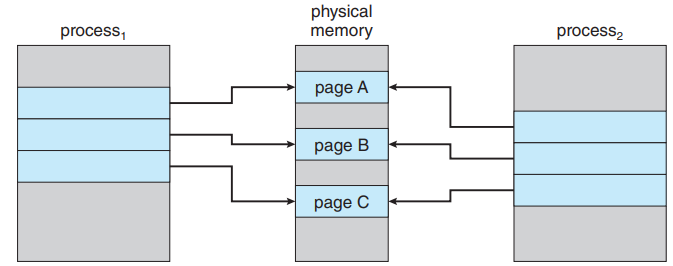
\includegraphics[width=12cm,height=3.2cm,keepaspectratio]{ch9_31.png}}
				\end{figure}
				\begin{figure}[ht!]
					\centering{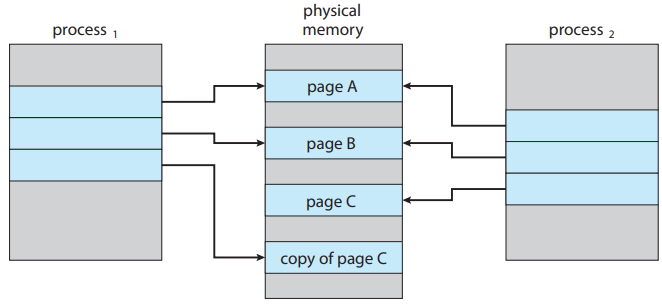
\includegraphics[width=12cm,height=3.7cm,keepaspectratio]{ch9_32.png}}
				\end{figure}
				Si noti inoltre che soltanto le pagine modificabili si devono contrassegnare come copy-on write, mentre
				quelle che non si possono modificare (per esempio, le pagine contenenti codice eseguibile) sono condivisibili dai processi genitore e figlio.
				\\Quando è necessaria la duplicazione di una pagina secondo la tecnica di copy-on-write, è importante capire da dove si attingerà la pagina libera necessaria. Molti SO forniscono, per queste richieste, un gruppo (pool) di pagine libere, che di solito si assegnano quando lo stack o lo heap di un processo devono espandersi, oppure proprio per gestire pagine da copiare su scrittura. L’allocazione di queste pagine di solito avviene secondo una tecnica nota come azzeramento su richiesta (\textbf{zero-fill-on-demand}); prima dell’allocazione si riempiono di zeri le pagine, cancellandone in questo modo tutto il contenuto precedente.
				\\Diverse versioni di UNIX (compreso Solaris e Linux) offrono anche una variante della chiamata di sistema fork() detta vfork() (per virtual memory fork). La vfork() offre un’alternativa all’uso della fork() con copiatura su scrittura. Con la vfork() il processo genitore viene sospeso e il processo figlio usa lo spazio d’indirizzi del genitore. Poiché la vfork() non usa la copiatura su scrittura, se il processo
				figlio modifica qualche pagina dello spazio d’indirizzi del genitore, le pagine modificate saranno visibili al processo genitore non appena riprenderà il controllo. È quindi necessaria molta attenzione nell’uso di vfork(), per assicurarsi che il processo figlio non modifichi lo spazio d’indirizzi del genitore. La chiamata di sistema vfork() è adatta al caso in cui il processo figlio esegua una exec() immediatamente dopo la sua creazione. Poiché non richiede alcuna copiatura delle pagine, la vfork() è un metodo di creazione dei processi molto efficiente, in alcuni casi impiegato per realizzare le interfacce shell in UNIX.

		\subsection{Sostituzione delle Pagine}
			Nelle descrizioni fatte finora sul tasso di page fault abbiamo supposto che ogni pagina poteva dar luogo al massimo a un fault, la prima volta in cui si effettuava un riferimento a essa. Tale rappresentazione tuttavia non è molto precisa. Se un processo di 10 pagine ne impiega effettivamente solo la metà, la paginazione su richiesta fa risparmiare l’I/O necessario per caricare le cinque pagine che non sono mai usate. Inoltre il grado di multiprogrammazione potrebbe essere aumentato eseguendo il doppio dei processi. Aumentando il grado di multiprogrammazione, si sovrassegna la memoria perché, nel caso i processi richiedano ulteriori pagine, la RAM potrebbe non essere sufficiente.
			\\Si consideri inoltre che la memoria del sistema non si usa solo per contenere pagine di programmi: le aree di memoria per l’I/O impegnano una rilevante quantità di memoria. Ciò può aumentare le difficoltà agli algoritmi di allocazione della memoria. Decidere quanta memoria assegnare all’I/O e quanta alle pagine dei programmi è un problema complesso. Alcuni sistemi riservano una quota fissa di memoria per l’I/o, altri permettono sia ai processi utenti sia al sottosistema di I/o di competere per tutta la memoria del sistema.
			\\La \textbf{sovrallocazione} (\textbf{over-allocation}) si può illustrare come segue. Durante l’esecuzione di un processo utente si verifica un page fault. Il SO determina la locazione del disco in cui risiede la pagina desiderata, ma poi scopre che la lista dei frame liberi è vuota: tutta la memoria è in uso. 
			\begin{figure}[ht!]
				\centering{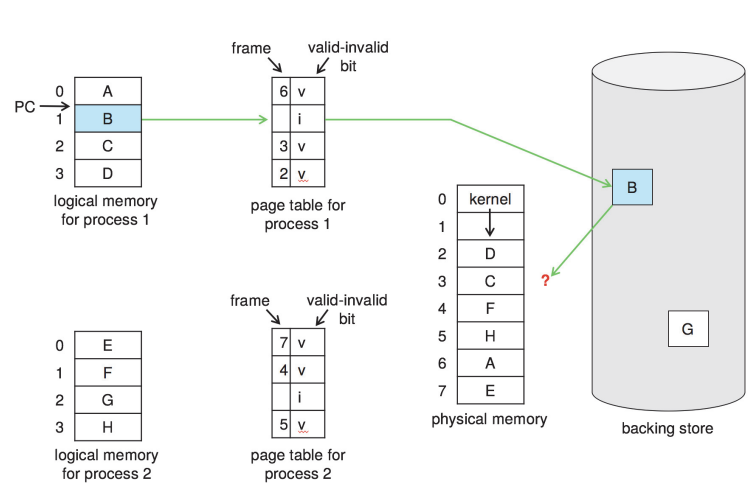
\includegraphics[width=12cm,height=3.7cm,keepaspectratio]{ch9_33.png}}
			\end{figure}
			\\A questo punto il SO può scegliere tra diverse possibilità, per esempio può terminare il processo utente. Tuttavia, la paginazione su richiesta è un tentativo che il SO fa per migliorare l’utilizzo e la produttività del sistema di calcolo. Gli utenti non dovrebbero sapere che i loro processi sono eseguiti su un sistema paginato. La paginazione deve essere logicamente trasparente per l’utente, quindi la terminazione del processo non costituisce la scelta migliore.
			\\In questa sede analizziamo l’opzione più comune: la \textbf{sostituzione delle pagine} (\textbf{page replacement}).

			\subsubsection{Page Replacement}
				La sostituzione delle pagine segue il seguente criterio: se nessun frame è libero, ne viene liberato uno attualmente inutilizzato. È possibile liberarlo scrivendo il suo contenuto nell’area di swap e modificando la tabella delle pagine (e tutte le altre tabelle) per indicare che la pagina non si trova più in memoria. 
				\begin{figure}[ht!]
					\centering{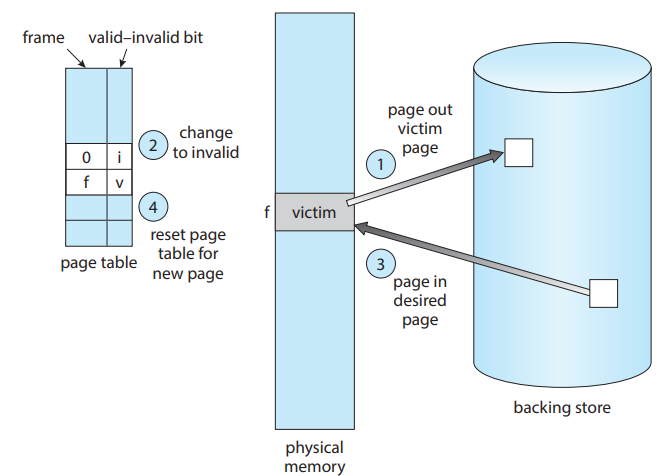
\includegraphics[width=12cm,height=4.2cm,keepaspectratio]{ch9_34.png}}
				\end{figure}
				\\Il frame liberato si può usare per memorizzare la pagina che ha causato il fault. Si modifica la procedura di servizio dell’eccezione di page fault in modo da includere la sostituzione della pagina:
				\begin{enumerate}
					\item s’individua la locazione su disco della pagina richiesta;
					\item si cerca un frame libero:
					\begin{enumerate}
						\item se esiste, lo si usa;
						\item altrimenti si impiega un algoritmo di sostituzione delle pagine per scegliere un frame vittima;
						\item si scrive la pagina “vittima” nel disco; si di conseguenza le tabelle delle pagine e quelle dei frame;
					\end{enumerate}
					\item si scrive la pagina richiesta nel frame appena liberato; si modificano le tabelle delle pagine e dei frame;
					\item si riprende il processo utente dal punto in cui si è verificato il page fault.
				\end{enumerate}
				Occorre notare che, se non esiste alcun frame libero sono necessari due trasferimenti di pagine, uno fuori e uno dentro la memoria. Questa situazione raddoppia il tempo di servizio del page fault e aumenta di conseguenza anche il tempo effettivo d’accesso.
				\\Questo sovraccarico si può ridurre usando un bit di modifica (modify bit o dirty bit). In questo caso l’hardware del calcolatore dispone di un bit di modifica, associato a ogni pagina (o frame), che viene posto a 1 ogni volta che nella pagina si scrive un byte, indicando che la pagina è stata modificata. Quando si sceglie una pagina da sostituire si esamina il suo bit di modifica; se è a 1, significa che quella pagina è stata modificata rispetto a quando era stata letta dal disco; in questo caso la pagina deve essere scritta nel disco. Se il bit di modifica è rimasto a 0, significa che la pagina non è stata modificata da quando è stata caricata in memoria, quindi non è necessario scrivere nel disco la pagina di memoria: c’è già. Questa tecnica vale anche per le pagine di sola lettura, per esempio pagine di codice binario. Queste pagine non possono essere modificate, quindi si possono rimuovere in ogni momento. Questo schema può ridurre in modo considerevole il tempo per il servizio del page fault, poiché dimezza il tempo di I/o, se la pagina non è stata modificata.
				\\La sostituzione di una pagina è fondamentale al fine della paginazione su richiesta, perché completa la separazione tra memoria logica e memoria fisica. Con questo meccanismo si può mettere a disposizione dei programmatori una memoria virtuale enorme con una memoria fisica più piccola. Senza la paginazione su richiesta, gli indirizzi utente si fanno corrispondere a indirizzi fisici e i due insiemi di indirizzi possono essere diversi. Tuttavia tutte le pagine di un processo devono ancora essere in memoria fisica. Con la paginazione su richiesta la dimensione dello spazio degli indirizzi logici non è più limitata dalla memoria fisica. Per esempio, un processo utente formato da 20 pagine si può eseguire in 10 frame semplicemente usando la paginazione su richiesta e un algoritmo di sostituzione per localizzare un frame libero ogni qual volta
				sia necessario. Se una pagina modificata deve essere sostituita, si copia nel disco il suo contenuto. Un successivo riferimento a quella pagina causa un’eccezione di page fault. In quel momento, la pagina viene riportata in memoria, eventualmente sostituendo un’altra pagina.
				Per realizzare la paginazione su richiesta è necessario risolvere due problemi principali: occorre sviluppare un algoritmo di allocazione dei frame e un algoritmo di sostituzione delle pagine. ossia, se sono presenti più processi in memoria, occorre decidere quanti frame vadano assegnati a ciascun processo. Inoltre, quando è richiesta una sostituzione di pagina, occorre selezionare i frame da sostituire. La progettazione di algoritmi idonei a risolvere questi problemi è un compito importante, poiché l’I/O nei dischi è molto oneroso. Anche miglioramenti minimi ai metodi di paginazione su richiesta apportano notevoli incrementi alle prestazioni del sistema.
				\\Esistono molti algoritmi di sostituzione delle pagine; probabilmente ogni sistema operativo ha il proprio schema di sostituzione. È quindi necessario stabilire un criterio per selezionare un algoritmo di sostituzione particolare; comunemente si sceglie quello con il minimo tasso di page fault.
				\\Un algoritmo si valuta effettuandone l’esecuzione su una particolare successione di riferimenti alla memoria e calcolando il numero di page fault. La successione dei riferimenti alla memoria è detta, appunto, successione dei riferimenti. Queste successioni si possono generare artificialmente (per esempio con un generatore di numeri casuali), oppure analizzando un dato sistema e registrando l’indirizzo di ciascun riferimento alla memoria. Quest’ultima opzione genera un numero elevato di dati, dell’ordine di un milione di indirizzi al secondo. Per ridurre questa quantità di dati occorre notare due fatti.
				\\Innanzitutto, per una pagina di dimensioni date, generalmente fissate dall’architettura del sistema, si considera solo il numero della pagina anziché l’intero indirizzo. In secondo luogo, se si ha un riferimento a una pagina p, i riferimenti alla stessa pagina immediatamente successivi al primo non generano page fault: dopo il primo riferimento, la pagina p è presente in memoria.
				\\Esaminando un processo si potrebbe per esempio registrare la seguente successione di indirizzi:
				\begin{center}
					0100, 0432, 0101, 0612, 0102, 0103, 0104, 0101, 0611, 0102, 0103,
					0104, 0101, 0610, 0102, 0103, 0104, 0101, 0609, 0102, 0105
				\end{center}
				che, a 100 byte per pagina, si riduce alla seguente successione di riferimenti:
				\begin{center}
					1, 4, 1, 6, 1, 6, 1, 6, 1, 6, 1
				\end{center}
				Per stabilire il numero di page fault relativo a una particolare successione di riferimenti e a un particolare algoritmo di sostituzione delle pagine, occorre conoscere anche il numero dei frame disponibili. Naturalmente, aumentando il numero di quest’ultimi diminuisce il numero di page fault. Per la successione dei riferimenti precedentemente esaminata, per esempio, dati tre o più blocchi di memoria avremmo solo tre fault: uno per il primo riferimento di ogni pagina. D’altra parte, se si dispone di un solo frame è necessaria una sostituzione per ogni riferimento, con il risultato di 11 page fault. In generale ci si aspetta una curva simile ala seguente:
				\begin{figure}[ht!]
					\centering{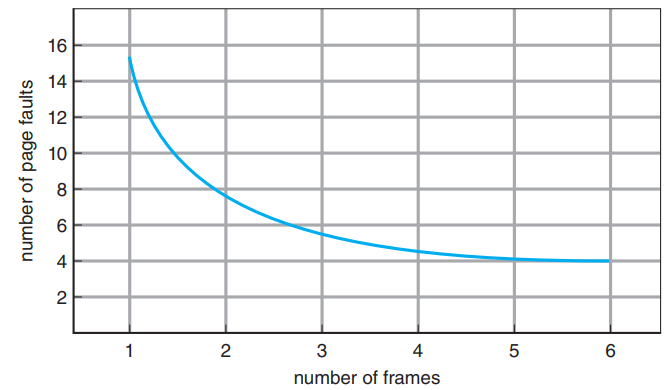
\includegraphics[width=12cm,height=4.2cm,keepaspectratio]{ch9_35.png}}
				\end{figure}
				\\Aumentando il numero dei frame, il numero di page fault diminuisce fino al livello minimo. Naturalmente aggiungendo memoria fisica il numero dei frame aumenta.
				\\Per illustrare gli algoritmi di sostituzione delle pagine impiegheremo la seguente successione di riferimenti:
				\begin{center}
					7, 0, 1, 2, 0, 3, 0, 4, 2, 3, 0, 3, 2, 1, 2, 0, 1, 7, 0, 1
				\end{center}
				per una memoria con tre frame.

			\subsubsection{Page Replacement Strategies}
				La frequenza dei page fault (numero di page fault sul numero totale di access) può essere espressa con la seguente formula:
				\begin{figure}[ht!]
					\centering{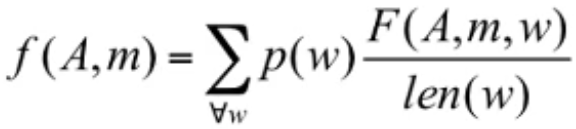
\includegraphics[width=12cm,height=1cm,keepaspectratio]{ch9_36.png}}
				\end{figure}
				\begin{itemize}
					\item \textbf{A}: algoritmo di page replacement;
					\item \textbf{m}: numero di frame disponibili (fisso e dedicato ad un dato processo);
					\item \textbf{p(w)}: probabilità che si debba accedere alla stringa di riferimento \textit{w};
					\item \textbf{F(A,m,w)}: numero di page fault generato da una certa stringa di riferimento \textit{w} usando un  algoritmo \textit{A} in un sistema con \textit{m} frame;
					\item \textbf{len(w)}: lunghezza della stringa di riferimento \textit{w}.
				\end{itemize}
				Come possiamo vedere dal seguente grafico, se ci sono pochi frame liberi, il tasso di page faul è alto. Se si hanno tanti frame la frequenza diminuisce, fino ad azzerarsi quando il numero di frame liberi è uguale a quello delle pagine del processo.
				\begin{figure}[ht!]
					\centering{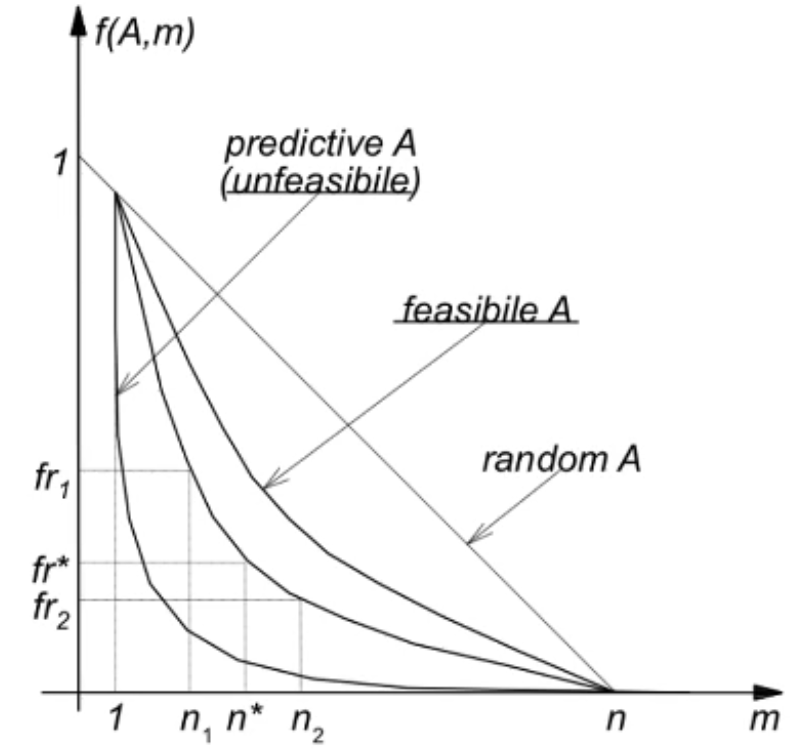
\includegraphics[width=12cm,height=4.4cm,keepaspectratio]{ch9_37.png}}
				\end{figure}
				\\Inoltre, possiamo notare che più l'algoritmo è stupido (la vittima da spostare viene scelta casualmente), più il grafico assomiglia a una retta.

			\subsubsection{FIFO Page Replacement}
				L’algoritmo di sostituzione delle pagine più semplice è un algoritmo FIFO: si crea una cosa FIFO in base all'ordine di arrivo delle pagine caricate in memoria e, se si deve sostituire una pagina, si seleziona quella presente in memoria da più tempo. Occorre notare che non è strettamente necessario registrare l’istante in cui si carica una pagina in memoria; infatti si può creare una coda FIFO di tutte le pagine presenti in memoria. In questo caso si sostituisce la pagina che si trova in testa alla coda. Quando si carica una pagina in memoria, la si inserisce nell’ultimo elemento della coda.
				\\Nella successione di riferimenti di esempio, i nostri tre frame sono inizialmente vuoti. I primi tre riferimenti (7, 0, 1) accusano ciascuno un page fault con conseguente caricamento delle relative pagine nei frame vuoti. Il riferimento successivo (2) causa la sostituzione della pagina 7, perché è stata caricata per prima in memoria. Questo processo prosegue come è illustrato:
				\begin{figure}[ht!]
					\centering{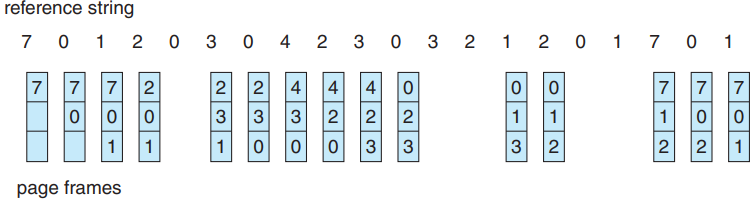
\includegraphics[width=12cm,height=4.4cm,keepaspectratio]{ch9_38.png}}
				\end{figure}
				\\Complessivamente si hanno 15 page fault.
				\\Questo algoritmo è facile da capire e da programmare; tuttavia la sue prestazioni non sono sempre buone. La pagina sostituita potrebbe essere un modulo di inizializzazione usato molto tempo prima e che non serve più, ma potrebbe anche contenere una variabile molto usata, inizializzata precedentemente, e ancora in uso.
				\\Occorre notare che anche se si sceglie una pagina da sostituire che è in uso attivo, tutto continua a funzionare correttamente anche se viene rallentata l'esecuzione del processo.
				\\Per illustrare i problemi che possono insorgere con l’uso di questo algoritmo, si consideri la seguente successione di riferimenti:
				\begin{center}
					1, 2, 3, 4, 1, 2, 5, 1, 2, 3, 4, 5
				\end{center}
				Nella seguente figura è illustrata la curva dei page fault per questa successione di riferimenti in funzione del numero dei frame disponibili:
				\begin{figure}[ht!]
					\centering{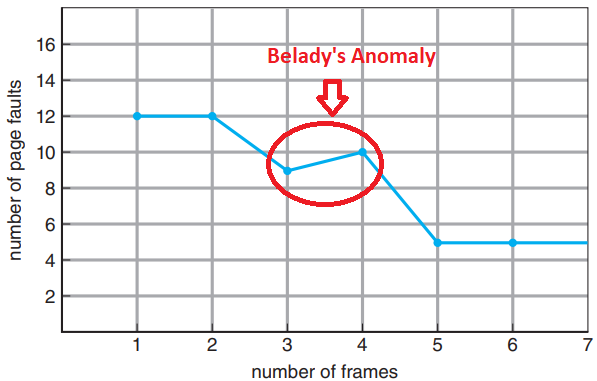
\includegraphics[width=12cm,height=4cm,keepaspectratio]{ch9_39.png}}
				\end{figure}
				\\Occorre notare che il numero dei page fault (10) per quattro frame è maggiore del numero dei page fault (9) per tre frame. Questo inatteso risultato è noto col nome di \textbf{anomalia di Belady}: con alcuni algoritmi di sostituzione delle pagine, il tasso di page fault può aumentare con il numero dei frame assegnati. A prima vista sembra logico supporre che fornendo più memoria a un processo le prestazioni di quest’ultimo migliorino. In alcune delle prime ricerche sperimentali si notò invece che questo presupposto non sempre è vero.

			\subsubsection{Algoritmo Ottimale di Page Replacement}
				In seguito alla scoperta dell’anomalia di Belady si è ricercato un algoritmo di page replacement ottimale. Tale algoritmo è quello che presenta il tasso minimo di page fault e non presenta mai l’anomalia di Belady. Questo algoritmo è stato chiamato OPT o MIN e consiste semplicemente nel sostituire la pagina che non verrà usata per il periodo di tempo più lungo.
				\\Per esempio, nella successione dei riferimenti d’esempio, l’algoritmo ottimale di sostituzione delle pagine produce nove page fault:
				\begin{figure}[ht!]
					\centering{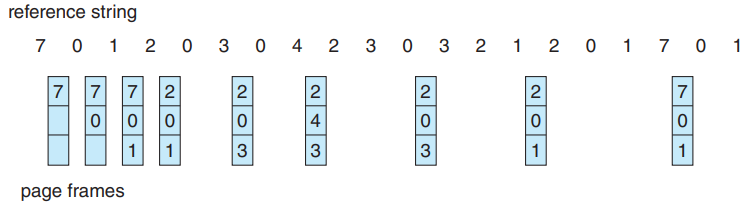
\includegraphics[width=12cm,height=4.4cm,keepaspectratio]{ch9_40.png}}
				\end{figure}
				\\Con sole nove page fault, la sostituzione ottimale risulta assai migliore di quella ottenuta con un algoritmo FIFO, dove i page fault erano 15. Ignorando i primi tre page fault, che si verificano con tutti gli algoritmi, la sostituzione ottimale è due volte migliore rispetto all’algoritmo FIFO; nessun algoritmo di sostituzione può gestire questa successione di riferimenti a tre blocchi di memoria con meno di nove page fault.
				\\Sfortunatamente l’algoritmo ottimale di sostituzione delle pagine è difficile da realizzare, perché richiede la conoscenza futura della successione dei riferimenti.

			\subsubsection{LRU Page Replacement}
				Se l’algoritmo ottimale non è realizzabile, è forse possibile realizzarne un’approssimazione. La distinzione fondamentale tra gli algoritmi FIFO e OPT, oltre quella di guardare avanti o indietro nel tempo, consiste nel fatto che l’algoritmo FIFO impiega l’istante in cui una pagina è stata caricata in memoria, mentre l’algoritmo OPT impiega l’istante in cui una pagina sarà usata. Usando come approssimazione di un futuro vicino un passato recente, si sostituisce la pagina che non è stata usata per il periodo più lungo. Il metodo appena descritto è noto come algoritmo LRU (Least Recently Used).
				\\La sostituzione LRU associa a ogni pagina l’istante in cui è stata usata per l’ultima volta. Quando occorre sostituire una pagina, l’algoritmo sceglie quella che non è stata usata per il periodo più lungo. Possiamo interpretare questa strategia come l’algoritmo ottimale di sostituzione delle pagine con ricerca all’indietro nel tempo, anziché in avanti.
				\\Il risultato dell’applicazione dell’algoritmo LRU alla successione dei riferimenti dell’esempio è la seguente:
				\begin{figure}[ht!]
					\centering{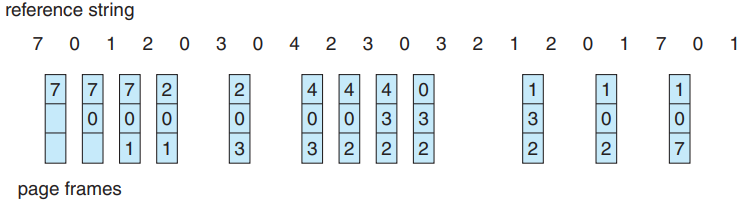
\includegraphics[width=12cm,height=4.4cm,keepaspectratio]{ch9_41.png}}
				\end{figure}
				\\L’algoritmo LRU produce 12 page fault, meglio della sostituzione FIFO (15).
				\\Vediamo un esempio più dettagliato:
				\begin{figure}[ht!]
					\centering{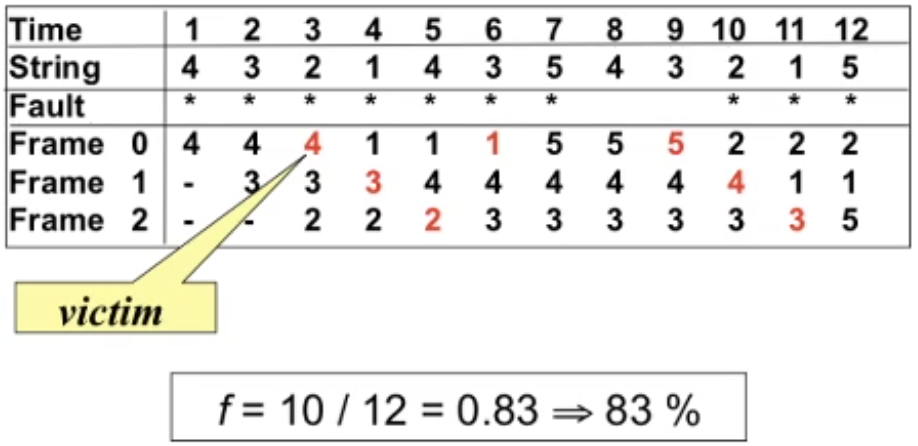
\includegraphics[width=12cm,height=4.4cm,keepaspectratio]{ch9_43.png}}
				\end{figure}
				\begin{itemize}
					\item \textbf{time}: tempo di accesso;
					\item \textbf{string}: stringa di riferimento;
				\end{itemize}
				Il criterio LRU si usa spesso come algoritmo di sostituzione delle pagine ed è considerato valido. Il problema principale riguarda la sua implementazione perché può richiedere una notevole assistenza da parte dell’hardware. Il problema consiste nel determinare un ordine per i frame definito dal momento dell’ultimo uso. Si possono realizzare le due seguenti soluzioni:
				\begin{itemize}
					\item \textbf{contatori}: nel caso più semplice, a ogni elemento della tabella delle pagine si associa un campo \textit{momento di utilizzo}, e alla CPU si aggiunge un contatore che si incrementa a ogni riferimento alla memoria. Ogni volta che si fa un riferimento a una pagina, si copia il contenuto del registro contatore nel campo \textit{momento di utilizzo} nella voce della page table relativa a quella pagina. Si sostituisce la pagina con il valore associato più piccolo. Questo schema implica una ricerca all’interno della tabella delle pagine per individuare la pagina usata meno recentemente, e una scrittura in memoria (nel campo \textit{momento di utilizzo} della tabella delle pagine) per ogni accesso alla memoria. I riferimenti temporali si devono mantenere anche quando, a seguito dello scheduling della CPU, si modificano le tabelle delle pagine. Occorre infine considerare l’overflow del contatore;
					\item \textbf{stack}: un altro metodo per la realizzazione della sostituzione delle pagine LRU prevede l’utilizzo di uno stack dei numeri delle pagine. Ogni volta che si fa un riferimento a una pagina, la si estrae dallo stack e la si colloca in cima a quest’ultimo. In questo modo, in cima allo stack si trova sempre la pagina usata per ultima, mentre in fondo si trova la pagina usata meno recentemente:
					\begin{figure}[ht!]
						\centering{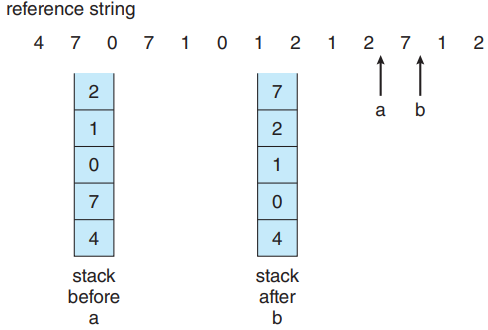
\includegraphics[width=12cm,height=4.4cm,keepaspectratio]{ch9_42.png}}
					\end{figure}
					\\Poiché gli elementi si devono estrarre dal centro dello stack, la migliore realizzazione si ottiene usando una lista doppiamente concatenata, con un puntatore all’elemento iniziale e uno a quello finale. Per estrarre una pagina dallo stack e collocarla in cima, nel caso peggiore è necessario modificare sei puntatori. Ogni aggiornamento è un po’ più costoso, ma per una sostituzione non si deve compiere alcuna ricerca: il puntatore dell’elemento di coda punta alla pagina LRU.
				\end{itemize}
				Né la sostituzione ottimale né quella LRU sono soggette all’anomalia di Belady. Entrambe appartengono a una classe di algoritmi di sostituzione delle pagine, chiamati \textbf{algoritmi a stack}, che non presenta l’anomalia di Belady. Un algoritmo a stack è un algoritmo per il quale è possibile mostrare che l’insieme delle pagine in memoria per \textit{n} frame è sempre un sottoinsieme dell’insieme delle pagine che dovrebbero essere in memoria per n + 1 frame. Per la sostituzione LRU, l’insieme di pagine in memoria è costituito delle \textit{n} pagine cui si è fatto riferimento più recentemente. Se il numero dei frame è aumentato, queste \textit{n} pagine continuano a essere quelle cui si è fatto riferimento più recentemente e quindi restano in memoria.

			\subsubsection{LRU Approximation Algorithms}
				Sono pochi i sistemi di calcolo che dispongono del supporto hardware per una vera sostituzione LRU delle pagine. Nei sistemi che non offrono alcun supporto hardware si devono impiegare altri algoritmi di sostituzione delle pagine, per esempio l’algoritmo FIFO. Molti sistemi tuttavia possono fornire un aiuto: un \textbf{bit di riferimento}. Il bit di riferimento a una pagina è impostato automaticamente dall’hardware ogni volta che si fa un riferimento a quella pagina, che sia una lettura o una scrittura su qualsiasi byte della pagina. I bit di riferimento sono associati a ciascun elemento della tabella delle pagine.
				\\Inizialmente, il SO azzera tutti i bit. Quando s’inizia l’esecuzione di un processo utente, l’hardware imposta a 1 il bit associato a ciascuna pagina cui si fa riferimento. Dopo qualche tempo è possibile stabilire quali pagine sono state usate semplicemente esaminando i bit di riferimento. Non è però possibile conoscere l’ordine d’uso. Questa informazione è alla base di molti algoritmi per la sostituzione delle pagine che approssimano LRU.

				\paragraph{Additional-Reference-Bits Algorithm\\}
					Ulteriori informazioni sull’ordinamento si possono ottenere registrando i bit di riferimento a intervalli regolari. È possibile conservare in una tabella in memoria con, ad esempio, un byte per ogni pagina. A intervalli regolari, per esempio di 100 millisecondi, un segnale d’interruzione del timer trasferisce il controllo al SO. Questo inserisce il bit di riferimento per ciascuna pagina nel bit più significativo del byte, shiftando gli altri bit a destra di 1 bit e scartando il bit meno significativo.
					\\Questi registri a scorrimento di 8 bit contengono la storia dell’utilizzo delle pagine relativo agli ultimi otto periodi di tempo. Se il registro a scorrimento contiene la successione di bit 00000000, significa che la pagina associata non è stata usata da otto periodi di tempo; a una pagina usata almeno una volta per ogni periodo corrisponde la successione 11111111 nel registro a scorrimento. Una pagina cui corrisponde la successione 11000100, è stata usata più recentemente di una pagina a cui corrisponde 01110111. Interpretando queste successioni di bit come interi senza segno, la pagina cui è associato il numero minore è la pagina LRU, e può essere sostituita. Si noti che l’unicità dei numeri non è garantita. Si possono sostituire tutte le pagine con il valore minore, oppure si può ricorrere a una selezione FIFO.
					\\Il numero dei bit può ovviamente essere variato: si sceglie secondo l’hardware disponibile per accelerarne al massimo la modifica. Nel caso limite tale numero si riduce a zero, lasciando soltanto il bit di riferimento. In questo caso l’algoritmo è noto come \textit{algoritmo di sostituzione delle pagine con seconda chance}.

				\paragraph{Algoritmo con Seconda Chance\\}
					L’algoritmo di base per la sostituzione con seconda chance è un algoritmo di sostituzione di tipo FIFO. Tuttavia, dopo aver selezionato una pagina, si controlla il bit di riferimento: se il suo valore è 0, si sostituisce la pagina; se è impostato a 1, si dà una seconda chance alla pagina e si passa alla successiva pagina FIFO.
					\\Quando una pagina riceve la seconda chance, si azzera il suo bit di riferimento e si aggiorna il suo istante d’arrivo al momento attuale. In questo modo, una pagina cui si offre una seconda chance non viene mai sostituita fiché tutte le altre pagine non siano state sostituite, oppure non sia stata data loro una seconda chance. Inoltre, se una pagina è usata abbastanza spesso, da mantenere il suo bit di riferimento impostato a 1, non viene mai sostituita.
					\\Un metodo per implementare l’algoritmo con seconda chance, detto anche a orologio (\textbf{clock}), è basato sull’uso di una coda circolare, in cui un puntatore (lancetta) indica qual è la prima pagina da sostituire. Quando serve un frame, si fa avanzare il puntatore finché non si trovi in corrispondenza di una pagina con il bit di riferimento 0; a ogni passo si azzera il bit di riferimento appena esaminato:
					\begin{figure}[ht!]
						\centering{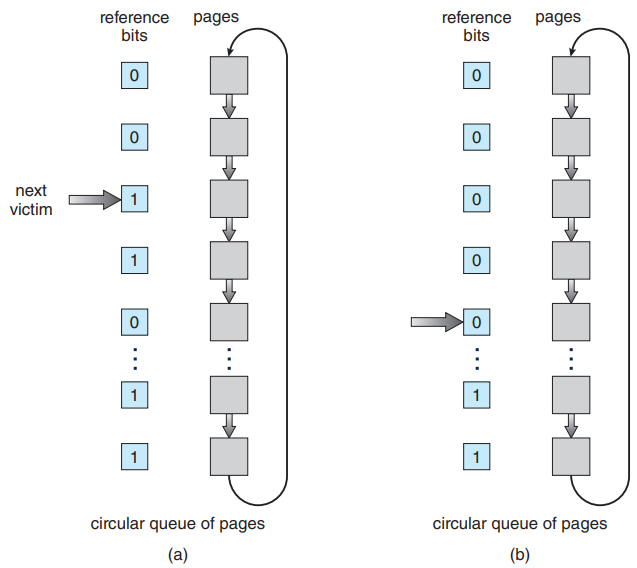
\includegraphics[width=12cm,height=5cm,keepaspectratio]{ch9_44.png}}
					\end{figure}
					\\Una volta trovata una pagina “vittima”, la si sostituisce e si inserisce la nuova pagina nella oda circolare nella posizione corrispondente. Si noti che nel caso peggiore, quando tutti i bit sono impostati a 1, il puntatore percorre un ciclo su tutta la coda, dando a ogni pagina una seconda chance. Prima di selezionare la pagina da sostituire, azzera tutti i bit di riferimento. Se tutti i bit sono a 1, la sostituzione con seconda chance si riduce a una sostituzione FIFO.
			
				\paragraph{Algoritmo con Seconda Chance Migliorato\\}
					L’algoritmo con seconda chance descritto precedentemente si può migliorare considerando i bit di riferimento e di modifica come una coppia ordinata, con cui si possono ottenere le seguenti quattro classi:
					\begin{enumerate}
						\item (0, 0) né recentemente usato né modificato – migliore pagina da sostituire;
						\item (0, 1) non usato recentemente, ma modificato – la pagina non così buona poiché prima di essere sostituita deve essere scritta in memoria secondaria;
						\item (1, 0) usato recentemente ma non modificato – probabilmente la pagina sarà presto usata nuovamente;
						\item (1, 1) usato recentemente e modificato – probabilmente la pagina sarà presto ancora usata e dovrà essere scritta in memoria secondaria prima di essere sostituita.
					\end{enumerate}
					Ogni pagina rientra in una di queste quattro classi. Alla richiesta di una sostituzione di pagina, si usa lo stesso schema impiegato nell’algoritmo a orologio, ma anziché controllare se la pagina puntata ha il bit di riferimento impostato a 1, si esamina la classe a cui la pagina appartiene e si sostituisce la prima pagina che si trova nella classe minima non vuota. Si noti che si può dover scandire la coda circolare più volte prima di trovare una pagina da sostituire.
					\\La differenza principale tra questo algoritmo e il più semplice algoritmo a orologio è che qui si dà la preferenza alle pagine modificate, al fine di ridurre il numero di I/ richiesti.

			\subsubsection{Counting Algotithms}
				Esistono molti altri algoritmi che si possono usare per la sostituzione delle pagine. Per esempio, si potrebbe usare un contatore del numero dei riferimenti fatti a ciascuna pagina, e sviluppare i due seguenti schemi:
				\begin{itemize}
					\item algoritmo di sostituzione delle pagine meno frequentemente usate (\textbf{Least Frequently Used}, \textbf{LFU}): richiede che si sostituisca la pagina con il conteggio più basso. La ragione di questa scelta è che una pagina usata attivamente deve avere un conteggio di riferimento alto. Si ha però un problema quando una pagina è usata molto intensamente durante la fase iniziale di un processo, ma poi non viene più usata. Poiché è stata usata intensamente il suo conteggio è alto, quindi rimane in memoria anche se non è più necessaria. Una soluzione può essere quella di spostare i valori dei contatori a destra di un bit a intervalli regolari, misurando l’utilizzo con un peso esponenziale decrescente;
					\item algoritmo di sostituzione delle pagine più frequentemente usate (\textbf{Most Frequently Used}, \textbf{MFU}); è basato sul fatto che, probabilmente, la pagina con il contatore più basso è stata appena inserita e non è stata ancora usata.
				\end{itemize}
				Le sostituzioni MFU e LFU non sono molto comuni, poiché la realizzazione di questi algoritmi è abbastanza onerosa; inoltre, tali algoritmi non approssimano bene la sostituzione OPT.

\end{document}